%!TEX root = Thesis.tex

\chapter{Ligand Synthesis and Properties}
\label{ch:ligands}

The \tBuxantphos{} ligand was first reported in 2005.\cite{Mispelaere2005} The original paper and several since then, have tested \tBuxantphos{} for use as an ancillary ligand in a range of different catalytic systems with mixed results.\cite{Dongol2007, Ohshima2009, Cabello2007, Friis2014, Dang2013, Liu2013c, Raoufmoghaddam2013, Haibach2013, Ashcroft2013, Behr2013, Raoufmoghaddam2013b, Zhan2012}  Despite the catalytic attention towards the \tBuxantphos{} ligand very little is known about the coordination chemistry or reasons for the very different catalytic activity compared to \Phxantphos{}.  Only one study comparing the coordination chemistry of the two ligands has been published.\cite{Partyka2010}  This study found that \tBuxantphos{} formed [Au(\tBuxantphos)][\ce{AuX2}] (X = \ce{Cl-}, \ce{Br-}, and \ce{I-}) complexes whereas \Phxantphos{} formed [\ce{(AuX)2}(\Phxantphos)].  A \trans-[Pd(\tBuxantphos)\ce{Cl2}] complex has been reported to the \gls{CSD} (CSD-XARXAR), while the analogous complex with \Phxantphos{} is \cis{}, indicating a difference in the coordination chemistry of the two ligands.\cite{Allen2002}  A series of rhodium complexes with \tBuxantphos{} has been published, though the analogous \Phxantphos{} complexes have not been investigated.\cite{Haibach2013}  

The original study into the \Phxantphos{} ligands investigated the effect of changing the bridging group in the backbone between \ce{CMe2}, \ce{SiMe2}, and \ce{S}.\cite{Kranenburg1995}  Changing this group subtly changes the natural bite-angle of the ligand and has been shown to impact the catalytic activity.\cite{Birkholz2009}  One derivative of \tBuxantphos{} in this position has been previously published with the \ce{CMe2} replaced by a \ce{C=CMe2}\cite{Marimuthu2012}  Given the much larger bite-angle of the \tBuxantphos{} ligands the impact of small changes may be very different to those observed with the \Phxantphos{} ligands.  This chapter presents a study into the synthesis of \tBusixantphos{} and \tButhixantphos, and an alternative synthesis of \tBuxantphos{}, followed by calculation of their natural bite-angles and the synthesis of some non-transition metal derivatives.  The goal of this chapter is to investigate the steric and electronic properties of the three \tBuxantphos{} ligands to form the foundation of knowledge, necessary to understand their coordination chemistry, which will be presented in later chapters.  

%The xantphos class of diphosphine ligands (Figure \ref{Xantphosligands}) are well-known in coordination chemistry and catalysis.  The bis(diphenylphosphino)xanthene ligands were the first ligands to be systematically studied for the impact of their bite-angle on catalysis.\cite{Kranenburg1995}  The derivatives showed significant variations in activity and selectivity for the rhodium catalysed hydroformylation of 1-octene.  Subsequently a large number of derivatives have been reported and they have been studied extensively in different catalytic reactions (for examples see \cite{Kamer2001, Asensio2010, Dieleman2001, Jahromi2012, Birkholz2009, Veen2000b}).  
%
%\begin{figure}[ht]
%\begin{center}
%\vspace{0.5cm}
%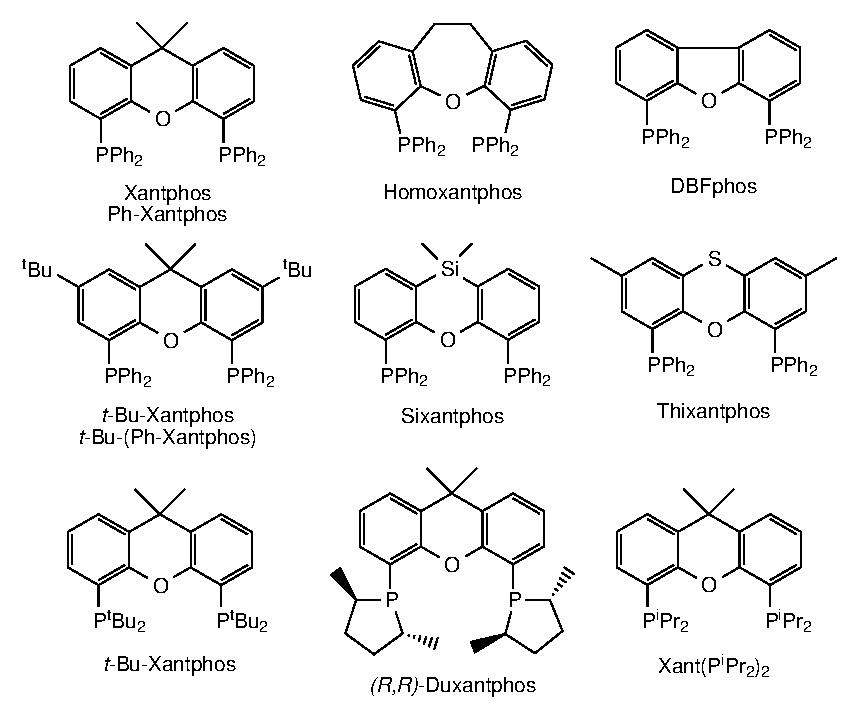
\includegraphics{../Figures/Xantphosligands.eps}
%\caption[Examples of the xantphos class of ligands]{Examples of the xantphos class of ligands showing naming and different sites for derivatisation.}
%\vspace{0.2cm}
%\label{Xantphosligands}
%\end{center}
%\end{figure}
%\vspace{0.2cm}
%
%%A vast number of wide bite-angle ligands based on a xanthene backbone have been synthesised since they were first reported in 1995.\cite{Kranenburg1995, Kamer2001, Esteruelas2011}  The bis-(diphenylphosphino)xanthene ligands were the first wide bite-angle ligands to be systematically studied.  Slight variations in the backbone led to changes in the calculated natural bite-angle.  The derivatives showed significant variations in activity in the rhodium catalysed hydroformylation reacti.  They have since been studied extensively in a range of different reactions \fixme{cite a review or something here} and a number of derivatives have been reported.  
%
%Derivatisation of xantphos has focussed mainly on two sites; the bridging group, to access a wider range of bite-angles, and the phosphine groups.  The original phenyl phosphines have been replaced with an array for different phosphines including cyclic groups\cite{Veen2000b}, chiral derivatives{\cite{Kamer2001} or changes for solubility.\cite{Buhling1997}  The phosphines have also been switched for different donors including phosphonites, amines, imines, arsines, thioethers and others.\cite{Veen2000b, Malaise2006, Goertz1998, Haaren2002} Further derivatives with substitutions on the aromatic backbone have also been reported, such as \emph{t}-Bu-(\Phxantphos), or sulfoxantphos.\cite{Goedheijt1998}  
%
%An analogue of xantphos has been reported with sterically bulky \tBu{} groups on the phosphines was first reported in 2005 as a ligand for the palladium catalysed cross-coupling of thiols and aryl bromides or triflates\cite{Mispelaere2005}.  \tBuXantphos{} has since been tested for activity in platinum catalysed amination of allylic alcohols,\cite{Ohshima2009} and the iron catalysed sp$^3$-sp$^3$ cross-coupling reactions of alkyl halides and alkyl Grignard reagents.\cite{Dongol2007}  However, in each of these cases the metal complexes were presumed to be formed in the catalytic mixtures and were not characterised.  
%
%To date, the only characterised transition metal complexes of \tBuxantphos{} are the series of gold halide complexes [Au(\tBuxantphos)\ce{][AuX2]} where X = Cl$^-$, Br$^-$ or I$^-$.\cite{Partyka2010}  In these structures the \tBuxantphos{} complexes were shown to have large bite angles of 143.0, 142.5 and 143.0\degrees{} for Cl$^-$, Br$^-$ and I$^-$ respectively.  When the same reaction was attempted with the \Phxantphos{} ligands, complexes of the type \ce{[(AuX)2}(\Phxantphos)] were formed.\cite{Pintado2004, Partyka2010}  These structures clearly indicate the difference between the phenyl and \tBu{} substituted xantphos ligands and the significant impact of the increased steric bulk of the \tBu{} groups on the bonding mode of the ligands.  
%
%The xantphos ligands are widely used in catalysis, but systems with \tBuxantphos{} have shown little activity.  This is an indication that the chemistry of the \tBuxantphos{} ligand is substantially different, as shown by the only characterised complexes of \tBuxantphos{} reported.\cite{Partyka2010}  Due to this difference in behaviour, further explorations into the coordination chemistry of \tBuxantphos{} and the reasons for this difference was deemed to be of scientific interest.  Furthermore, the difference in the activity of complexes with \Phxantphos{}, \Phsixantphos{} and \Phthixantphos{} has been previously reported.  Although complexes of \tBuxantphos{} have shown little catalytic activity, altering the bridging group, and thus the bite-angle, can have a significant impact on the coordination behaviour and the catalytic activity of the complexes produced.  This chapter reports the synthesis of \tBusixantphos{}, \tButhixantphos{} and \tBuxantphos{} along with some of the non-transition metal reactivity of these diphosphines.  

%As these gold complexes are the only examples of characterised tBu-xantphos metal complexes and the phenyl xantphos ligands are so widely utilised the tBu-xantphos ligand system was chosen for further study.  

\section{Ligand Synthesis}\label{section:ligandsynthesis}

In 2002 van Leeuwen \emph{et al.} reported their unsuccessful attempts to synthese \tBuxantphos{} from either the dilithiated xanthene backbone or starting with 9,9-dimethyl-4,5-bis(dichlorophosphino)xanthene, suggesting that steric crowding from the presence of two \tBu{} groups on a single phosphorus atom prevented the successful coupling.\cite{Zuideveld2002}  However, in 2005 a synthesis of \tBuxantphos{} from the dilithiated backbone was reported.\cite{Mispelaere2005}  This synthesis involves lithiation of the xanthene backbone using \emph{n}-butyllithium and \gls{TMEDA} in heptane, followed by addition of \ce{ClP^{t}Bu2} and heating at 60 \degC{} for 24 hours, generating the product in 38\% isolated yield (Scheme \ref{scheme:Otherligandsynthesis}).

\begin{scheme}[ht]
\begin{center}
\vspace{0.5cm}
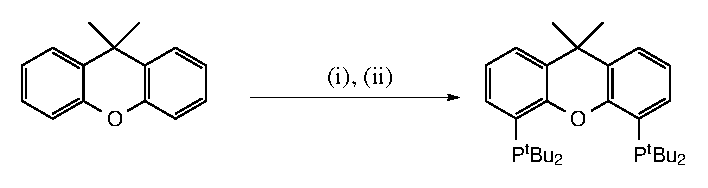
\includegraphics{../Schemes/Otherligandsynthesis.eps}
\caption[Literature synthesis of \tBuxantphos]{Literature synthesis of \tBuxantphos{} in heptane.\cite{Mispelaere2005}  \emph{Reagents and conditions:} (i) \emph{n}-BuLi, \gls{TMEDA}, 15 h, heptane. (ii): \ce{ClP^{t}Bu2}, 60 \degC, 24 h.}
\vspace{0.2cm}
\label{scheme:Otherligandsynthesis}
\end{center}
\end{scheme}
\vspace{0.2cm}

%The previously reported synthesis for tBu-xantphos\cite{Mispelaere2005} involved lithiation of the backbone in heptane followed by the addition of chlorodi-\emph{tert}-butyl phosphine and heating to 60\degrees C for 24 hours.  The reportedly air-stable product was obtained and recrystallised from n-propanol in 38\% yield.  Attempts to use this method for the synthesis of tBu-thixantphos yielded a mixture of products.\fixme{check this}

Attempts to utilise the literature method for the synthesis of \tBuxantphos{}\cite{Mispelaere2005} to synthesise \tButhixantphos{} resulted in a number of unidentifiable products.  An alternative method using a potassium \emph{tert}-butoxide$/$\emph{n}-butyllithium ``superbase'' formed a mixture of products from which separation attempts were unsuccessful.  This superbase mixture forms significant amounts of organopotassium compounds, which are more active metallating agents than their organolithium counterparts.  However, organopotassium compounds are also more active in cleavage of ethers.\cite{Bhatt1983}  Hence the mixture of products may result from cleavage of the ether or thioether bridges resulting in undesired compounds.

%This reference doesn't actually cover organopotassium, just sodium and lithium.

The syntheses of \tButhixantphos{}, \tBusixantphos{} and \tBuxantphos{} were successfully achieved by adaptation of the reported synthesis of the \Phxantphos{} ligands\cite{Kranenburg1995}.  This method involves the dilithiation of the backbone using \emph{sec}-butyl\-lithium and \gls{TMEDA}, followed by reaction with chlorodi-\emph{tert}-butyl phosphine (Scheme \ref{Ligandsynthesis}).  Unlike the \Phxantphos{} synthesis which is complete in 16 hours, the synthesis of the \tBu{} ligands required extended periods.  The reactions were allowed to proceed until no further change was determined by NMR spectroscopy (typically seven days).  NMR analysis of the crude reaction mixture showed the presence of both the mono and diphosphine.  The diphosphine was isolated as white crystals by recrystallisation from \emph{n}-propanol.  The remaining \emph{n}-propanol solution of the monophosphine could be reduced to dryness and then reused for a second lithiation and reaction with chlorodi-\emph{tert}-butyl phosphine to produce more of the desired diphosphine.  

 %carried out in diethyl ether with \gls{TMEDA} using \emph{sec}-butyllithium, added at -78\degrees C followed by addition of the chlorodi-\emph{tert}-butyl phosphine and stirring for 16 hours.  After 16 hours of reaction the NMR spectra showed a mixture of mono and di-substituted products.  The reaction was allowed to proceed until no further change was determined by NMR (typically 7 days).  The reaction invariably produced a mixture of mono and diphosphine.  The diphosphine was separated from the monophosphine by-product by recrystallisation from hot n-propanol and cooling at -16\degC.  The diphosphine was obtained in \fixme{yield} as white crystals.  

\begin{scheme}[ht]
\begin{center}
\vspace{0.5cm}
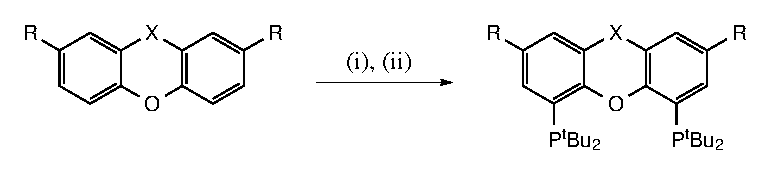
\includegraphics{../Schemes/Ligandsynthesis.eps}
\caption[Ligand synthesis]{Synthesis of \tBuxantphos{} (X = \ce{CMe2}, R = H), \tButhixantphos{} (X = S, R = Me) and \tBusixantphos{} (X = \ce{SiMe2}, R = H).  \emph{Reagents and conditions:} (i)  \emph{sec}-BuLi, \ce{Et2O} -78\degC{} $\rightarrow$ RT, 24 hours(ii) \ce{ClP^{t}Bu2}, -78\degC{} $\rightarrow$ RT, 7 days.}
\vspace{0.2cm}
\label{Ligandsynthesis}
\end{center}
\end{scheme}
\vspace{0.2cm}

The size of the \tBu{} groups leads to difficulties in the synthesis of the \tBuxantphos{} ligands.  Reaction with one equivalent of chlorodi-\emph{tert}-butyl phosphine to form the monophosphine is clean and rapid, occurring overnight.  However, the steric hindrance of the monophosphine results in a much slower second addition, requiring extended reaction times to achieve significant conversion.  When the reaction is allowed to proceed for longer than one week, no additional conversion is observed.  This is likely due to degradation of either the lithiated monophosphine or the \emph{sec}-butyllithium before the second lithiation can occur.  Over extended periods organolithium reagents cleave diethyl ether resulting in alkanes, alkenes, and lithium ethoxide (Scheme \ref{Organolithium}).\cite{Bhatt1983, Gilman1954}  \emph{sec}-Butyllithium has been shown to completely react with diethyl ether in one day.\cite{Gilman1954}  Although the reaction between diethyl ether and phenyllithium is slower (half-time of 100 hours), the extended reaction periods required for the second phosphine addition mean that this degradation pathway may limit the yield of the diphosphine.

%Between \emph{n}-butyllithium the reaction occurs with a half time of 6 days at 25\degC{}.\fixme{ref}  Although an aryl lithium with an ortho oxygen group would be expected to reaction more slowly with the diethyl ether this is one possible pathway for reaction.  \fixme{does this happen in THF}  

%This is likely a result of the steric bulk of the \emph{tert}-butyl groups hindering the second addition reaction.  However, over time organolithium reagents react with diethyl ether generating lithium ethoxide and ethene (Scheme \ref{Organolithium}).  This reaction occurs with a half time of 6 days at 25\degC{} for \emph{n}-butyllithium.  This is likely the reason for the lack of observed reaction after periods of one week.

\begin{scheme}[ht]
\begin{center}
vspace{0.5cm}

\includegraphics{../Schemes/Organolithium.eps}
\caption[Reaction of \emph{n}-butyllithium with diethyl ether]{Reaction of \emph{n}-butyllithium with diethyl ether}
\vspace{0.2cm}
\label{Organolithium}
\end{center}
\end{scheme}
\vspace{0.2cm}

In order to promote the dilithiation, a pre-formed \emph{sec}-butyllithium$/$\gls{TMEDA} complex was added to a solution of the backbone.  An initial colour change to yellow (\tButhixantphos{} and \tBusixantphos) or green (\tBuxantphos) was observed, indicative of monolithiation.  After stirring overnight this changed to red or yellow respectively.  This colour change gives a clear indication of successful dilithiation.  In order to favour the diphosphine over the monophosphine, the lithiated backbone was then added slowly to an ethereal solution of chloro-di-\emph{t}-butylphosphine.  Although a mixture of the mono and diphosphine was always obtained, this order of addition was found to be more successful, resulting in increased yields.

The synthesis of these ligands utilises directed \emph{ortho} metallation as first described independently by Gilman and Wittig in 1939 and 1940 respectively.\cite{Gilman1939, Wittig1940} Directed \emph{ortho} metallation uses a heteroatom that can coordinate to the organolithium reagent, thereby directing it to the \emph{ortho} sites.  In the synthesis of the \tBuxantphos{} ligands the ether linkage can act as a director for the lithiation.  Once lithiated, the electron density on the oxygen stabilises the lithiated site against degradation.  For \tBuxantphos{} and \tBusixantphos{} the oxygen is the only atom present with lone pairs of electrons and thus the lithiation occurs exclusively in the desired positions \emph{ortho} to the oxygen.  However, the precursor to \tButhixantphos{}, phenoxathiin, contains both an ether and a thioether group, both of which can act as \emph{ortho}-directors.\cite{Organolithiummethods}  Previous research has shown that in the presence of both ether and thioether groups the lithiation will occur \emph{ortho} to the oxygen.\cite{Turck1997}  Once the first lithiation has taken place the oxygen is less likely to contribute significantly to the second lithiation.  For \tBuxantphos{} and \tBusixantphos{} the influence of the oxygen is still sufficient for the second lithiation to occur in the other \emph{ortho} position.  However for phenoxathiin the thioether acts as a second directing group and the lithiation occurs \emph{ortho} to the sulfur (Scheme \ref{scheme:transthixantphos}).  The addition of methyl groups in the positions \emph{meta} to the thioether prevents the sulfur atom from acting as a director, resulting in the desired \tButhixantphos{} ligand.  

\begin{scheme}[ht]
\begin{center}
\vspace{0.5cm}
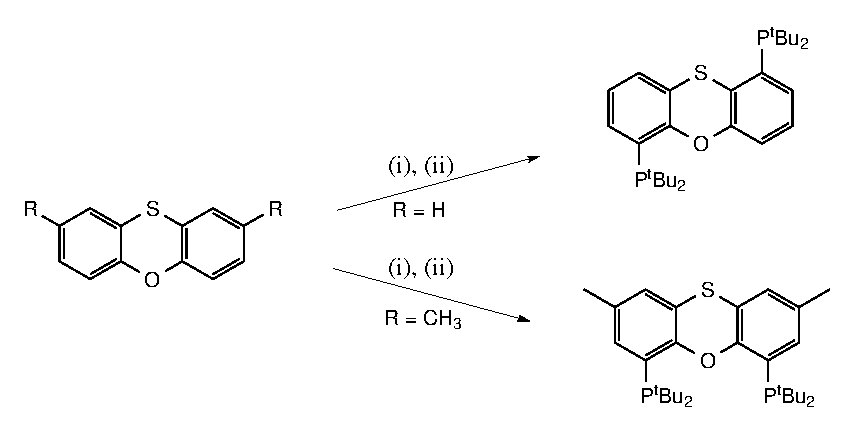
\includegraphics{../Schemes/Transthixantphos2.eps}
\caption[Influence of methyl groups on the synthesis of \tButhixantphos]{Influence of methyl groups on the synthesis of \tButhixantphos. \emph{Reagents and conditions:} (i)  \emph{sec}-BuLi, \ce{Et2O}, 24 hours, (ii) \ce{ClP^{t}Bu2}, 24 hours.}
\vspace{0.2cm}
\label{scheme:transthixantphos}
\end{center}
\end{scheme}
\vspace{0.2cm}

The \tBuxantphos{} ligand obtained using \emph{sec}-butyllithium$/$TMEDA in diethyl ether had \proton{} and \carbon{} NMR spectra consistent with the literature (Table \ref{table:ligandNMRdata}).\cite{Mispelaere2005} However the \phosphorus{} chemical shift differed by 2.2~ppm (10.2~ppm in this study compared to 12.4 ppm).  The NMR spectra for the reported and the synthesised samples were both obtained in \ce{CDCl3} and referenced to an external 85\% \ce{H3PO4} standard.  Hence the reason for this difference is unclear.  However, as the remainder of the NMR and other characterisation data is consistent, it is likely that the two compounds are identical and a typographical error or otherwise was made in the preparation of the earlier paper.



%The methyl groups on the aromatic system of \tButhixantphos{} was found to be important.  The attempted synthesis of a \tButhixantphos{} without methyl groups resulted in substitution ortho to the oxygen and ortho to the sulfur in a transoid configuration (Scheme \ref{Transthixantphos}).  It is likely that using three equivalents of \emph{sec}-butyllithium results in lithiation in three positions, the two ortho to the oxygen and one ortho to the sulfur.  The first addition of phosphine attacks one ortho to the oxygen.  This creates increased steric hindrance at the second site ortho to oxygen so the second equivalent of phosphine preferentially attacks in the least hindered site; ortho to the sulfur.  \fixme{this paragraph may in fact just be lies}.  The oxygen in the bridge of all three ligands acts as a directing group to promote lithiation in the ortho position.  However in the case of \tButhixantphos{} the sulfur can also act as a directing group (though less strongly that the oxygen) this leads to competition for the lithiation site and requires the methyl on the backbone to provide steric hindrance and prevent lithiation ortho to the sulfur.  This difficulty was not encountered with either the \tBuxantphos{} or \tBusixantphos{} ligands.  The carbon and silicon groups are not able to interact with the lithium and promote ortho lithiation so the lithiation occurs exclusively ortho to the oxygen. \fixme{see directed ortho lithiation for more info}



%However, the synthesis of \tBusixantphos{} was not problem free.  Given the extended reaction times necessary to obtain the diphosphines, the formed diphosphine is in solution with large volumes of lithium chloride for a substantial amount of time.  NMR analysis of the synthesis of \tBusixantphos{} showed the formation of a significant amount of a compound with a single peak in the \phosphorus{} NMR spectrum at 15 ppm.  No new peaks were observed in the \proton{} NMR spectrum.  However, due to the similarity in the spectra to those of \tBusixantphos H+ we propose that this compound is [Li\tBusixantphos]Cl.  The compound is unchanged through extensive water washing.  Attempts to remove the lithium ion using the lithium specific chelating agent, 12-crown-4, were unsuccessful.  Reaction with tetrafluoroboric acid in order to exchange the lithium for a proton led to the formation of a new species the nature of which could not be determined.  The formation of [Li\tBusixantphos]Cl results in a significant loss of product for the synthesis of \tBusixantphos{} resulting in lower yields than those for \tBuxantphos{} and \tButhixantphos{}.

%It was found the \tBusixantphos{} tended to capture lithium ions between the two phosphorus atoms.  These lithium ions were tightly bound and were retained through several cycles of washing with water.  The nature of this species was confirmed by reaction with a sample of the pure ligand with lithium chloride, resulting in the same product.  \fixme{do this} Attempts to react the lithiated \tBusixantphos{} with tetrafluoroboric acid to exchange the lithium ion for a proton was unsuccessful and instead resulted in possibly a boron trifluoride bound between the two phosphines.\fixme{check this with boron NMR etc.}  Attempts to remove the lithium using the lithium specific chelating agent, 12-crown-4, were unsuccessful.  Due to the inability to remove the lithium this represents a source of significant loss of product for the synthesis of \tBusixantphos{} resulting in lower yields than those for \tBuxantphos{} and \tButhixantphos{}.

The NMR data of the newly reported \tButhixantphos{} and \tBusixantphos{} ligands are consistent with expectations (Table \ref{table:ligandNMRdata}).  In both cases a plane of symmetry reduces the number of signals, showing a single peak in the \phosphorus{} NMR.  The \phosphorus{} NMR chemical shifts for the \tBusixantphos{} and \tButhixantphos{} ligands are observed as singlets at 8.4 and 9.5 ppm respectively.  The \proton{} NMR signals for the aromatic system are as expected, with two singlets present for \tButhixantphos, and a doublet, a doublet of doublets and a triplet observed for \tBusixantphos{} and \tBuxantphos.  The chemical shift of the methyl substituents differs for each ligand, as expected.  In \tBusixantphos{} the dimethylsilyl group appears at 0.46 ppm, close to the tetramethylsilane reference.  In \tBuxantphos{} the bridgehead methyls appear at 1.57 ppm, within the typical range for organic methyl groups.  The methyl groups in \tButhixantphos{} are evident at 2.25 ppm, consistent with methyl substituents attached to aryl rings.  

\begin{table}[ht]
\small
\caption[Selected NMR data for \tBuxantphos{} ligands]{Selected NMR data for \tBuxantphos{} ligands in \ce{CDCl3}}
\label{table:ligandNMRdata}
\begin{center}
\begin{tabular}{l c c c c c c}
	\toprule
	~ & \bfseries{\phosphorus} & \multicolumn{5}{c}{\bfseries{\proton}} \\
	\cmidrule(lr){2-2} \cmidrule(lr){3-7}
	\bfseries{Diphosphine} & \bfseries{$\delta/$ppm} & \bfseries{$\delta$ \ce{^{t}Bu}$/$ppm} & \bfseries{$\delta$ Me$/$ppm} & \multicolumn{3}{c}{\bfseries{$\delta$ Ar$/$ppm}} \\
	\midrule
	\tBuXantphos\cite{Mispelaere2005}	& 12.4 & 1.21--1.26 & 1.57 & 7.02 & 7.38 & 7.60 \\
	\tBuXantphos{} (this work) 		& 10.2 & 1.21--1.25 & 1.57 & 7.03 & 7.38 & 7.60 \\
	\tBuThixantphos				& 9.5 & 1.22--1.24 & 2.25 & 6.88 & 7.29 & \\
	\tBuSixantphos					& 8.4 & 1.29 vt & 0.46 & 7.12 & 7.53 & 7.87\\ 
	\bottomrule{}
\end{tabular}
\end{center}
\end{table}

The \proton{} NMR data for the \tBuxantphos{} ligands show a complex \ce{X18A}A'\ce{X18}' spin system for the \tBu{} protons. In a system where the two A atoms (in this case the phosphorus atoms) are strongly coupled, this leads to interaction between the three-bond and five-bond couplings (e.g. when the phosphorus atoms are in a \trans configuration in a metal complex) resulting in a virtual triplet.\cite{Harris1964}  In the \tBuxantphos{} ligands there is no atom between the phosphorus atoms so we would expect a three-bond and a nine-bond coupling.  A nine-bond coupling is an extremely remote coupling which we would expect to be negligible.  Based on previous reports,\cite{Harris1964, Abraham1961} this peak shape with two sharp outer lines and a broad inner peak occurs when the difference between the short- and long-range couplings is very small but not zero.  For this to occur the phosphines must have some degree of through-space spin-spin coupling through their lone pairs of electrons (for a review of non-bonded spin-spin coupling see Hierso\cite{Hierso2014}).  This is further supported by the difference in the \proton{} NMR spectra of the three ligands; the central peak is sharpest for \tBusixantphos{} followed by \tButhixantphos{}.  For \tBuxantphos{} some further detail can be seen indicating that this has the weakest through-space coupling.  This trend is consistent with the expected changes in the distance between the phosphines upon varying the backbone, which will impact the degree of through-space coupling that can occur, and therefore the difference in the short and long-range coupling constants.

%include spectra showing the tBu peak?

\section{Bite-Angle Calculations}
\label{section:biteangle}

The steric and electronic properties of diphosphine ligands determine their complexation behaviour with transition metals and can influence the reactivity of the complexes, particularly impacting the activity and selectivity in catalytic transformations.\cite{Freixa2003, Birkholz2009}  The xantphos class of ligands were initially investigated their consistent electronic properties and steric bulk meant that the impact of the bite-angle on rhodium catalysed hydroformylation could be studied exclusively.\cite{Kranenburg1995}  Consequently, a number of studies have investigated the bite-angle impact on a variety of catalytic conversions (for examples see\cite{Kranenburg1995b, Haaren2001b, Dudle2011b, Fanjul2013, Birkholz2009}).  However, it has since been determined that the bite-angle is a result of both the steric and electronic properties of the ligand.\cite{Freixa2003}

The natural bite-angle (\natbiteangle) was first described by Casey and Whiteker\cite{Casey1990} as a theoretically determined parameter to indicate the preferred chelation angle of diphosphine ligands irrespective of the metal they are coordinating to.  These are determined computationally by optimising the geometry of a complex with a rhodium atom at 2.315 \si{\angstrom} and measuring the resulting P-Rh-P angle.  The crystallographic bite-angle for a given complex can be measured from the crystal structure.  The original development of the natural bite-angle parameter included a comparison of the natural bite-angle for seven different ligands and crystallographic bite-angles for one transition metal complex of each ligand.  The two bite-angles were found to be correlated in accordance with the equation $\Theta$\sub{exp} = 0.98\natbiteangle{} + 2.13 (R = 0.92).\cite{Casey1990}  Another study in 2009 showed that for a range of diphosphines the crystallographically determined bite-angles have a narrow range, which is close to the calculated natural bite-angle.\cite{Dierkes1999}  This study did not however, determine a correlation between the two.

Despite the ubiquity of the natural bite-angle within diphosphine chemistry, only two studies have investigated whether the natural bite-angle has proven to be an apt predictor of the crystallographically determined bite-angle.\cite{Casey1990, Dierkes1999}  One of these only used one complex for each ligand and the other did not calculate the mathematical relationship between the two.  A large number of new crystal structures have also been reported since the studies were published in the 1990's.\cite{Allen2002}  In order to establish whether the natural bite-angle is still an apt predictor of the crystallographic bite-angle, almost 25 years after the original publication, the relationship between the two was investigated using data from the 2014 \gls{CSD}.\cite{Allen2002}  The results are summarised in Table \ref{table:biteangles} and Figure \ref{Biteanglegraph}.  The median crystallographic bite-angle was used to decrease the influence of outliers on the results.  The natural and experimental bite-angles show a good correlation described by the equation $\Theta$\sub{exp} = 1.10 \natbiteangle - 5.70 (R\superscript{2} = 0.92).  Some of the experimental and natural bite-angles that are most relevant to this work show significant differences (for example \tBuxantphos{} \natbiteangle{} = 140\degrees, experimental = 153.317\degrees{}, and \Phsixantphos{} \natbiteangle{} = 109\degrees{}, experimental = 99.165\degrees).  This may be due to the low numbers of structures available for these ligands (four and five respectively) at which point the metals used will have a significant impact. 

\begin{table}[htbp]
\small
\caption[Crystallographic bite-angles for diphosphine ligands]{Crystallographic bite-angles for diphosphine ligands, taken from the \gls{CSD}.\cite{Allen2002}} 
\label{table:biteangles}
\begin{center}
\begin{tabular}{c c c c c c}
	\toprule
	~~\bfseries{Diphosphine}~~ & \bfseries{Structures} & \bfseries{P-P ($\si{\angstrom}$)} & \bfseries{Range (\degrees)} & \bfseries{Bite-Angle (\degrees)} & \bfseries{$\beta$\sub{n} (\degrees)}\\
	\midrule
	dppm			& 384	& 2.718	& 62.757--77.706 	& 71.062 	& 73	\\
	dppe				& 1939	& 3.095	& 71.073--92.926	& 83.818	& 78 \\
	dppp				& 3237	& 3.308	& 83.333--105.420	& 92.181	& 86 \\ 
	BINAP			& 146	& 3.296	& 85.9820--115.666	& 91.925	& 92 \\
	dppb				& 127	& 3.391	& 89.447--111.491	& 94.240	& 99 \\
	DPEphos			& 101	& 3.844	& 96.094--158.531	& 112.691	& 102 \\
	\PhXantphos		& 65		& 3.908	& 98.829--153.134	& 108.535	& 111 \\
	BISBI			& 4		& 4.079	& 103.533--151.951	& 124.789 & 123 \\
	\PhSixantphos		& 5		& 3.691 	& 95.250--152.149	& 99.165 & 109 \\
	\PhThixantphos		& 3		& 4.021	& 109.528--155.050	& 111.724	& 110 \\
	\tBuxantphos		& 4		& 4.527	& 152.302--153.456 & 153.317 & 140 \\
	dpp-benzene		& 116	& 3.101	& 74.380--92.499	& 84.900	& 83\\
	dppn				& 25		& 3.176	& 79.867--93.270	& 86.864	& 82 \\
	dppx				& 19		& 3.569	& 90.045--106.186	& 102.636	& 90 \\
	dbpe				& 109	& 3.200	& 83.989--95.949	& 90.369	& 87	\\
	dbpp				& 12		& 3.503	& 94.556--104.857	& 99.175	& 99	\\
	dbpx				& 10		& 3.634	& 98.758--107.255	& 101.881	& 101 \\
	\bottomrule{}
\end{tabular}
\end{center}
\end{table}

\begin{figure}[htb]
\begin{center}
\vspace{0.5cm}
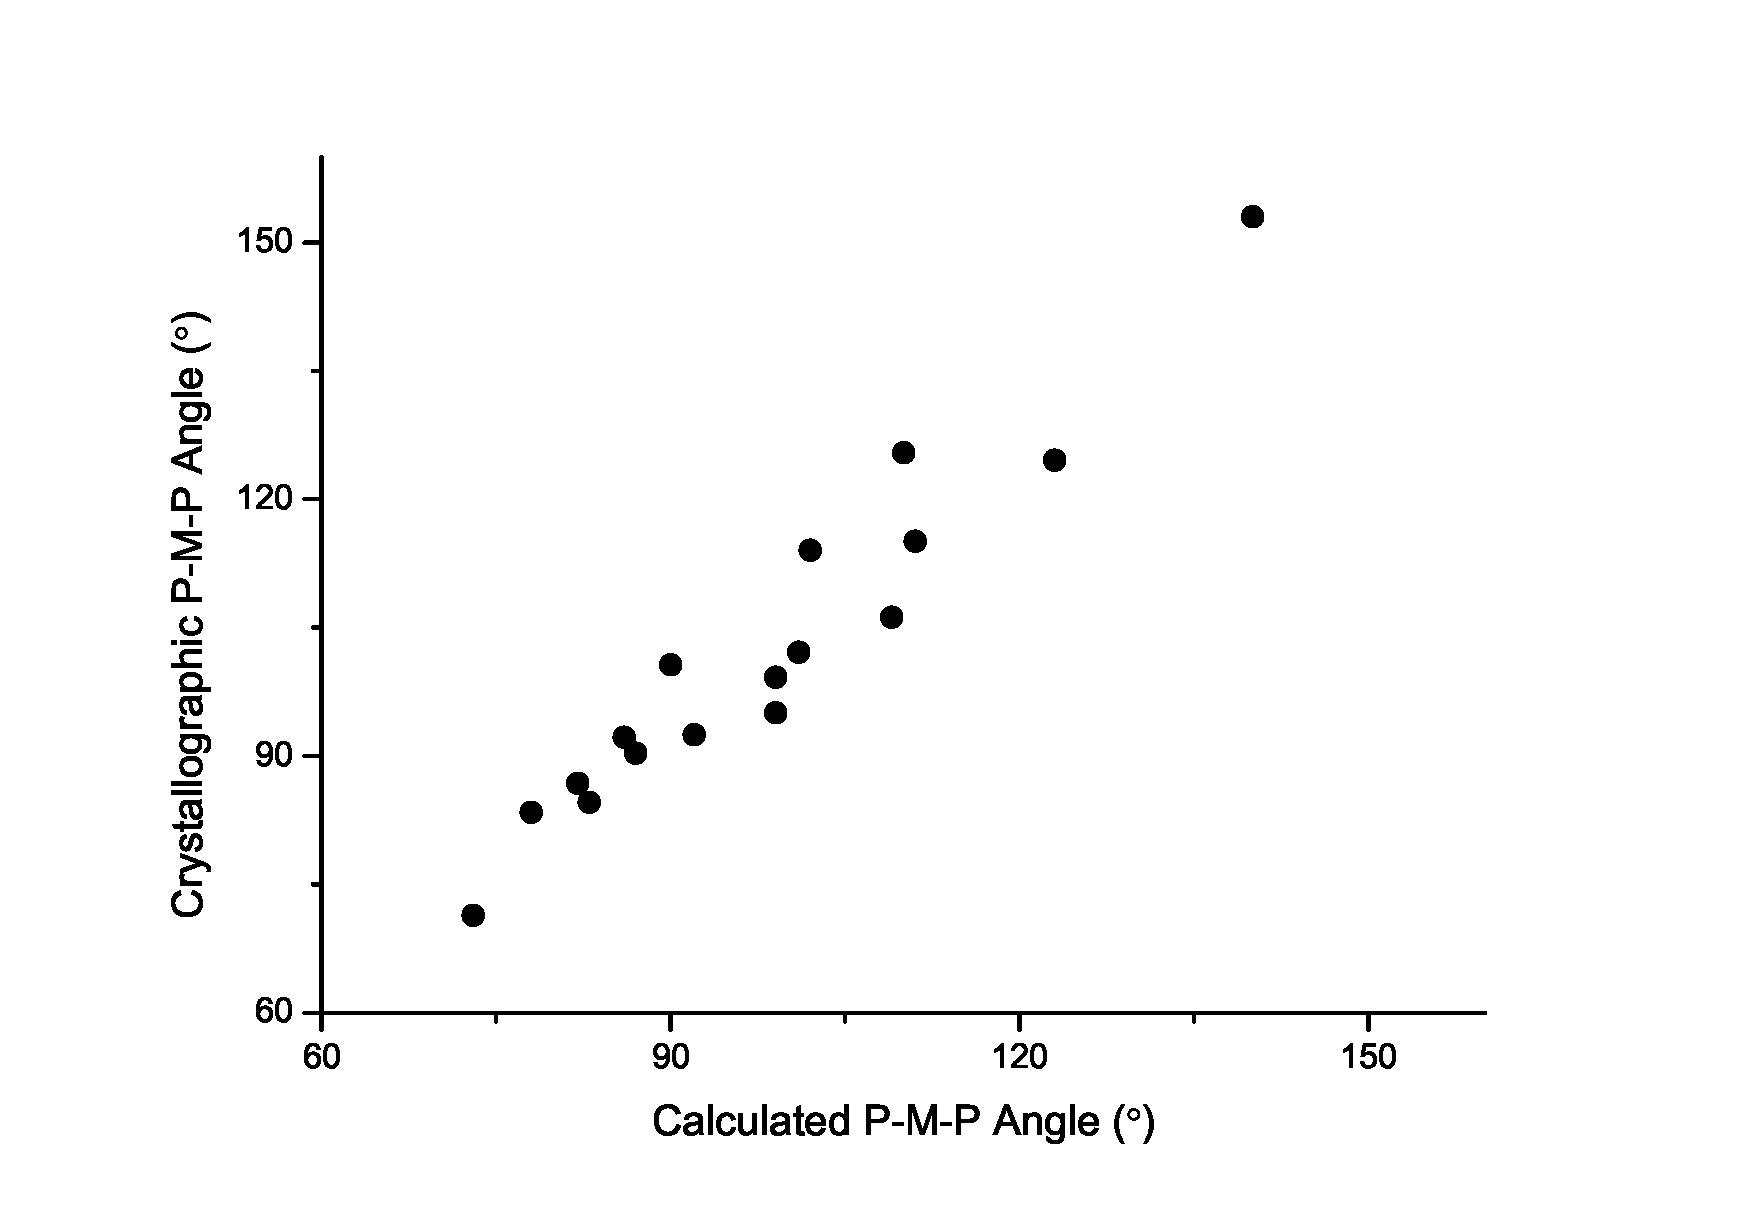
\includegraphics[width=\textwidth]{../Figures/Biteanglegraphorigin.eps}
\caption[Comparison of the natural and crystallographic bite-angles]{Comparison of the natural and crystallographic bite-angles.  Trendline $\Theta$\sub{exp} = 1.10 \natbiteangle - 5.70 (R\superscript{2} = 0.92).}
\vspace{0.2cm}
\label{Biteanglegraph}
\end{center}
\end{figure}
\vspace{0.2cm}

In order to determine the potential differences between the \tBuxantphos{} and \Phxantphos{} ligands, the natural bite-angles of the three \tBuxantphos{} ligands were calculated.  Previously the \tBuxantphos{} bite-angle was calculated using molecular mechanics, however molecular mechanics has previously been reported as overestimating the bite-angles for diphosphines with bulky alkyl substituents, like the \tBu{} groups in the \tBuxantphos{} ligands.\cite{Dierkes1999}  As the bite-angles of the \tBuxantphos{} ligands are an integral part of the current study \gls{DFT} was utilised to reduce the likelihood of overestimation.  The angles for the \Phxantphos{} ligands were also calculated to allow for a comparison between the \gls{DFT} and molecular mechanics methods.  The structures were optimised using the B3LYP functional,\cite{Becke1993, Lee1988, Vosko1980, Stephens1994} with the def2-TZVP basis set.\cite{Andrae1990, Weigend2005} using a Rh-P distance of 2.315 \si{\angstrom}.  The resulting bite-angles along with those published using molecular mechanics are given in Table \ref{table:biteanglescalculated}.  The values calculated using DFT and molecular mechanics are slightly larger for the \Phxantphos{} ligands.  The trend is consistent and molecular mechanics techniques can overestimate the impact of $\pi$-stacking in molecules with phenyl rings.  The value for \tBuxantphos{} using DFT is much smaller than the literature value calculated with molecular mechanics.  However, molecular mechanics is known to overestimate the bite-angles of bulky diphosphines which may account for this difference.\cite{Dierkes1999}

%These show good agreement with those calculated using molecular mechanics.  Given the good agreement of our DFT obtained values and the literature values we continued by calculating the bite-angles for the two new ligands \tButhixantphos{} and \tBusixantphos{}.  A number of different bite-angles have been reported for the \Phxantphos{} series, due to different computational set-ups.  

\begin{table}[ht]
\small
\caption[Natural bite-angles of xantphos ligands]{Natural bite-angles of xantphos ligands.  Molecular mechanics values taken from the literature.\cite{Kranenburg1995}}
\label{table:biteanglescalculated}
\begin{center}
\begin{tabular}{l c c}
	\toprule
	\bfseries{Diphosphine}	&\bfseries{Molecular Mechanics (\degrees)}&\bfseries{DFT (\degrees)}\\
	\midrule		
	\PhSixantphos		&108.7	&111.89	\\
	\PhThixantphos		&109.4	&\fixme{value}\\
	\PhXantphos		&111.7	&114.18	\\	
	\tBuSixantphos		&		&126.80	\\
	\tBuThixantphos	&		&126.98	\\
	\tBuXantphos		&140		&127.56	\\
	\bottomrule{}
\end{tabular}
\end{center}
\end{table}

%  including allylic alkylations\cite{Haaren1999}, rhenium catalysed hydrogenation\cite{Dudle2011b} and the palladium catalysed hydromethoxycarbonylation of ethene.\cite{Fanjul2013}  
%reviews have investigated whether the bite-angle impact is 

The natural bite-angles for the \tBuxantphos{} series of ligands are much larger than for the \Phxantphos{} ligands.  Given that the remainder of the ligands are unchanged, this effect is due to the impact of the \tBu{} groups.  \emph{Tert}-butyl groups are more electron-donating than the phenyl groups so the phosphorus atoms will have more electron density resulting in an electrostatic repulsion of the two phosphorus atoms.  The \tBu{} groups also have a larger steric impact than the planar phenyl rings.  This would result in a larger bite-angle as the steric bulk of the \tBu{} substituents pushes the two phosphorus atoms further apart.  The trend between the two groups is the same with the \ce{CMe2} bridged ligands having the largest \biteangle{}s and the \ce{SiMe2} bridged having the smallest.  However, the range for the \tBuxantphos{} ligands (0.76\degrees{}) is much smaller than for the \Phxantphos{} ligands (2.3\degrees{}).  This suggests that the \tBu{} substituents are the main contributing factor to the bite-angle and the small changes in the bridging group have a smaller effect because the sterics of the \tBu{} groups dominates.  

The bite-angles of the \tBuxantphos{} ligands are likely to have a significant impact on their coordination chemistry.  The phenyl ligands form a range of complexes favouring \cis-chelation in square-planar and octahedral complexes, although \emph{trans} square planar complexes have been reported\cite{Petocz2004}.  With bite-angles of 126.8--127.6\degrees{} the \tBuxantphos{} ligands may prefer bis-equatorial positions in trigonal bipyramidal complexes with angles close to 120\degrees.  However, the bite-angles are halfway between the \cis{}- and \trans{}-coordination angles for square-planar complexes, which may result in mixtures of products.  Mixtures of \cis{} and \trans{} isomers have been reported for palladium \Phxantphos{} complexes, so the ratio between the two geometries may favour \trans{}-coordination for the \tBuxantphos{} ligands.\cite{Zuideveld2002, Petocz2004} Diphosphine ligands that exhibit exclusive \trans-chelation have been described in a review as ``elusive''.\cite{Freixa2008}  

%\PhXantphos{} itself can form \trans-chelates\cite{Petocz2004}, however these form as a mixture of the \cis and \trans isomers rather than forming as the pure \trans isomer.  Only a small number of these \trans-chelates for \Phxantphos{} have been reported compared to the majority of complexes where the \cis-chelate forms.  A limited number of ligands exist that can form \trans-chelates, however, rarer are those that do not form \cis-chelates and rarer still are the truly \trans-chelating ligands with a bite-angle of 180\degrees{} and an undistorted coordination plane. 

%The wide bite-angles of the \tBuxantphos{} ligands may also result in interesting catalytic activity.  Previously reported uses of \tBuxantphos{} have added the ligand to a metal precusor and formed the catalyst in situ.  However platinum(II), palladium(II) and iron prefer either square-planar or octahedral coordination and if the \tBuxantphos{} ligand coordinated in a \trans{} configuration this may prevent the reductive elimination of other ligands.  Hence although \tBuxantphos{} has not shown activity in catalytic systems to date, these ligands may find more use in systems with metals able to form tetrahedral, trigonal planar, or pyramidal structures such as silver or rhodium, or platinum and palladium(0).

%\section{Oxidation}

%Although previous literature reports \tBuxantphos\cite{Mispelaere2005} as an air-stable solid, this was not the case for at least \tButhixantphos.  The ligands are resistant to oxidation and can be handled in the air for short periods.  However, storage in the air leads to slow oxidation.  

%The ligands appear to be more stable to oxidation using hydrogen peroxide than \Phxantphos{}.  Although the \tBuxantphos{} ligands oxidise slowly in the air which \Phxantphos{} does not; attempts to directly oxidise using a large excess of hydrogen peroxide in acetone requires extended periods of reflux while \Phxantphos{} undergoes complete oxidation after only 1 hour at room temperature.\cite{Jahromi2012}

%However problems were encountered with this as the thioether bridge is also susceptible to oxidation.  As such attempts to oxidise the phosphines of \tButhixantphos resulted in oxidation of one of the phosphine arms and the thioether bridge to a sulfoxide or sulfone resulting in a mixture of products.  

\section{Basicity}
\label{section:ligands:basicity}

Spectroscopic analysis of the \tBuxantphos{} ligands in \ce{CDCl3} showed a small amount of an impurity, characterised by a new peak in the \phosphorus{} NMR spectra and an unusual spin system downfield of the aromatic signals in the \proton{} NMR spectra.  The amount of the impurity increased over time, suggesting that the ligands were reacting with the solvent.  Chloroform is known to undergo slow degradation forming hydrochloric acid.\cite{Yano1977}  Tertiary phosphines can act as Br\o nsted bases, forming phosphonium ions that can be used as components in catalytic reactions.\cite{Netherton2001}  Hence, the identity of these compounds as phosphonium salts seemed likely.

%As discovered during the synthesis of \tBusixantphos{} the ligands have the ability to coordinate small cations.  Although only \tBusixantphos{} coordinated lithium to any significant degree during the synthesis, all three of the ligands are significantly acid sensitive and will react with any adventitious proton source resulting in the protonation at one of the phosphines.  Although stable for short periods in deutero-chloroform, over time chloroform produces hydrochloric acid \emph{via} photo-degradation which readily protonates the ligands

The three \tBuxantphos{} ligands react with the strong acids \ce{HCPh(SO2CF3)2} (\pKa = 2.0 in DMSO) or \ce{H2C(SO2CF3)2} (\pKa = 2.4 in DMSO), resulting in immediate formation of a phosphonium salt (Scheme \ref{Protonation}).\cite{Koppel2000}  These acids are useful as they are non-hygroscopic solids allowing for accurate stoichiometry.  Addition of excess acid results in the same product; no evidence for an additional protonation was observed.  The NMR data is consistent with the data for the impurity observed in the synthesis of the \tBuxantphos{} ligands, indicating that the impurity is [(\tBuxantphos)H\ce{]+}.

\begin{scheme}[ht]
\begin{center}
\vspace{0.5cm}
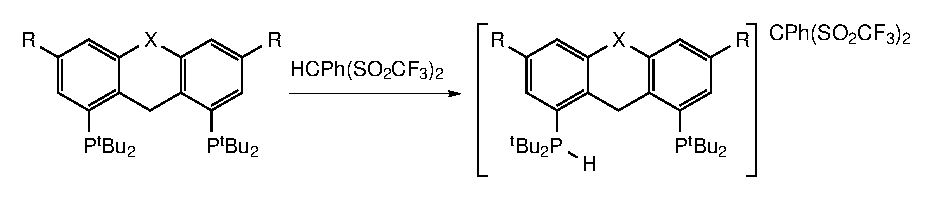
\includegraphics{../Schemes/Protonation.eps}
\caption[Protonation of the ligands using a strong acid]{Protonation of the ligands using a strong acid, in C6D6.}
\label{Protonation}
\end{center}
\end{scheme}
\vspace{0.2cm}

Selected NMR data for the phosphonium salts [(\tBuxantphos)\ce{H]+} with the three ligands is given in Table \ref{table:protonatedNMR}.  A broad singlet is present in the \phosphorus{} NMR spectra for the three phosphonium ions, shifted slightly downfield from the free ligand.  The \proton{} and \carbon{} NMR spectra show half the expected number of aromatic signals, and only one signal for the \tBu{} protons and the quaternary and terminal carbons.  This indicates that although the expected complex is asymmetric the system is undergoing a dynamic process such that the two halves of the molecule are equivalent on the NMR timescale.  The most likely process is the exchange of the proton between the two phosphorus atoms.  The \proton{} NMR spectra all show a complex spin system of the type XAA\textprime{}X\textprime{} for the phosphonium proton, which is further evidence for the dynamic exchange of the proton between the two phosphorus atoms.  

\begin{table}[htbp]
\caption[Selected NMR data for [(\tBuxantphos)H{]}\ce{CH(SO2CF3)2}]{Selected NMR data for the [(\tBuxantphos)H{]}\ce{CH(SO2CF3)2} compounds in \ce{CDCl3}.}
\label{table:protonatedNMR}
\small
\begin{center}
\begin{tabular}{l c c c}
	\toprule{}
	~~ & \multicolumn{2}{c}{\bfseries{\phosphorus}} & \bfseries{\proton}\\
	\cmidrule(lr){2-3} \cmidrule(lr){4-4}
	\bfseries{Ligand}&\bfseries{$\delta/$ppm}&\bfseries{$\Delta\delta/$ppm}& \bfseries{\ce{H+}$\delta/$ppm}\\
	\midrule
	\tBuSixantphos		& 14.3	& 5.9 	& 9.57 \\
	\tBuThixantphos 	& 15.8	& 6.3		& 8.99 \\
	\tBuXantphos		& 17.4	& 7.2		& 8.57 \\
	\bottomrule{}
\end{tabular}
\end{center}
\end{table}

The difference in the rate of exchange of the proton in the three compounds is clearly shown by their \phosphorus{} and \proton{} NMR spectra.  The \phosphorus{} NMR signal is sharpest for \tBusixantphos{} followed by \tButhixantphos{} while \tBuxantphos{} has a very broad signal.  This indicates that the exchange is fastest for \tBusixantphos{} and slowest for \tBuxantphos{}.  The \proton{} NMR spectra (Figure \ref{Protonatedligandsnmr}) show an XAA\textprime{}X\textprime{} spin system for the phosphonium proton.  The signal appears most like a virtual triplet for \tBusixantphos{}, implying very little difference in the coupling constants of the proton with each phosphorus.  For \tButhixantphos{} the central peak has broadened slightly, while in \tBuxantphos{} the central peak is very broad, indicating that the difference in the two coupling constants is increasing.  The chemical shift of the phosphonium proton is different  for the three systems (\tBusixantphos{} = 9.57, \tButhixantphos{} = 8.99 and \tBuxantphos{} = 8.57~ppm).  This indicates that the \tBusixantphos{} proton is less shielded and thus has a faster rate of exchange, while the \tBuxantphos{} proton is the most shielded and has the slowest rate of exchange.  This trend is consistent with the bite-angles of the ligands.  \tBuSixantphos{} has the smallest bite-angle, so the two phosphorus atoms are closer resulting in a lower barrier to exchange, whilst \tBuxantphos{} has the largest bite-angle and thus the slowest exchange.  

%The \phosphorus{} NMR spectrum has a single broad signal at 15.8 ppm showing a downfield shift of 6.3 ppm upon protonation.  In the \proton{} NMR spectrum the phosphonium proton comes at 9.0~ppm much higher than other phosphonium ions.  In addition the proton appears as an unusual signal in a 1:2:1 ratio with two sharp outer peaks and a broad inner peak.  The \phosphorus{}, \proton{} and \carbon{} spectra show half of the expected peaks indicating a plane of symmetry through the central bridge of the molecule.  However, the signal for the phosphonium proton only integrates for a single proton.  Together with the broadness of the \phosphorus{} and some of the \carbon{} signals this indicates a dynamic system in solution with proton exchange between the two phosphorus atoms.   \fixme{this data is for the sulfur bridged ligand should I include stuff for silicon as well?} 

\begin{figure}[htb]
\begin{center}
\vspace{0.5cm}
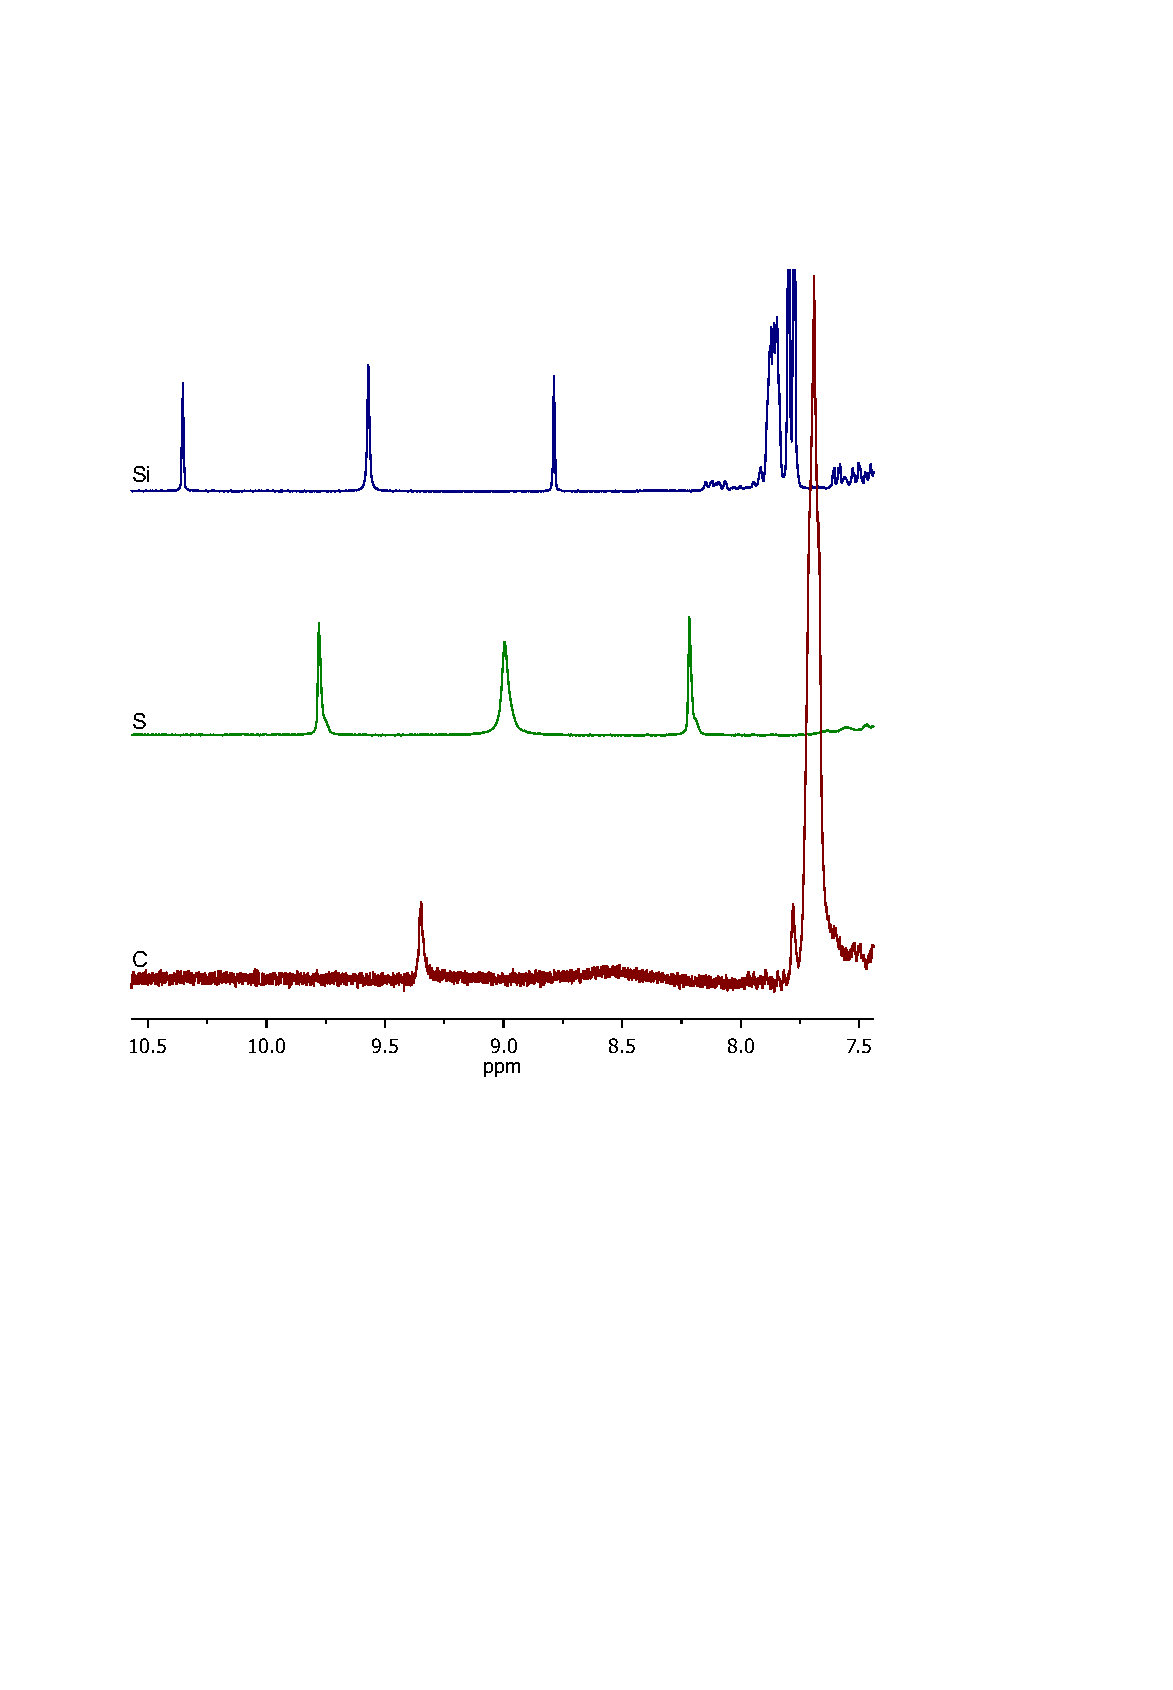
\includegraphics[scale = 0.8, trim = 1.5cm 10cm 4.5cm 5cm, clip]{../NMR/Phosphoniumstacked.eps}
\caption[\proton{} NMR spectra for the [(\tBuxantphos)H\ce{]+} ions]{\proton{} NMR spectra in \ce{CDCl3} at 20 \degC{} for [(\tBusixantphos)H\ce{]+}, [(\tButhixantphos)H\ce{]+}, and [(\tBuxantphos)H\ce{]+} (Si, S and C respectively) showing the P-H region}
\vspace{0.2cm}
\label{Protonatedligandsnmr}
\end{center}
\end{figure}
\vspace{0.2cm}

%\begin{figure}[htp]
%\begin{center}
%\vspace{0.5cm}
%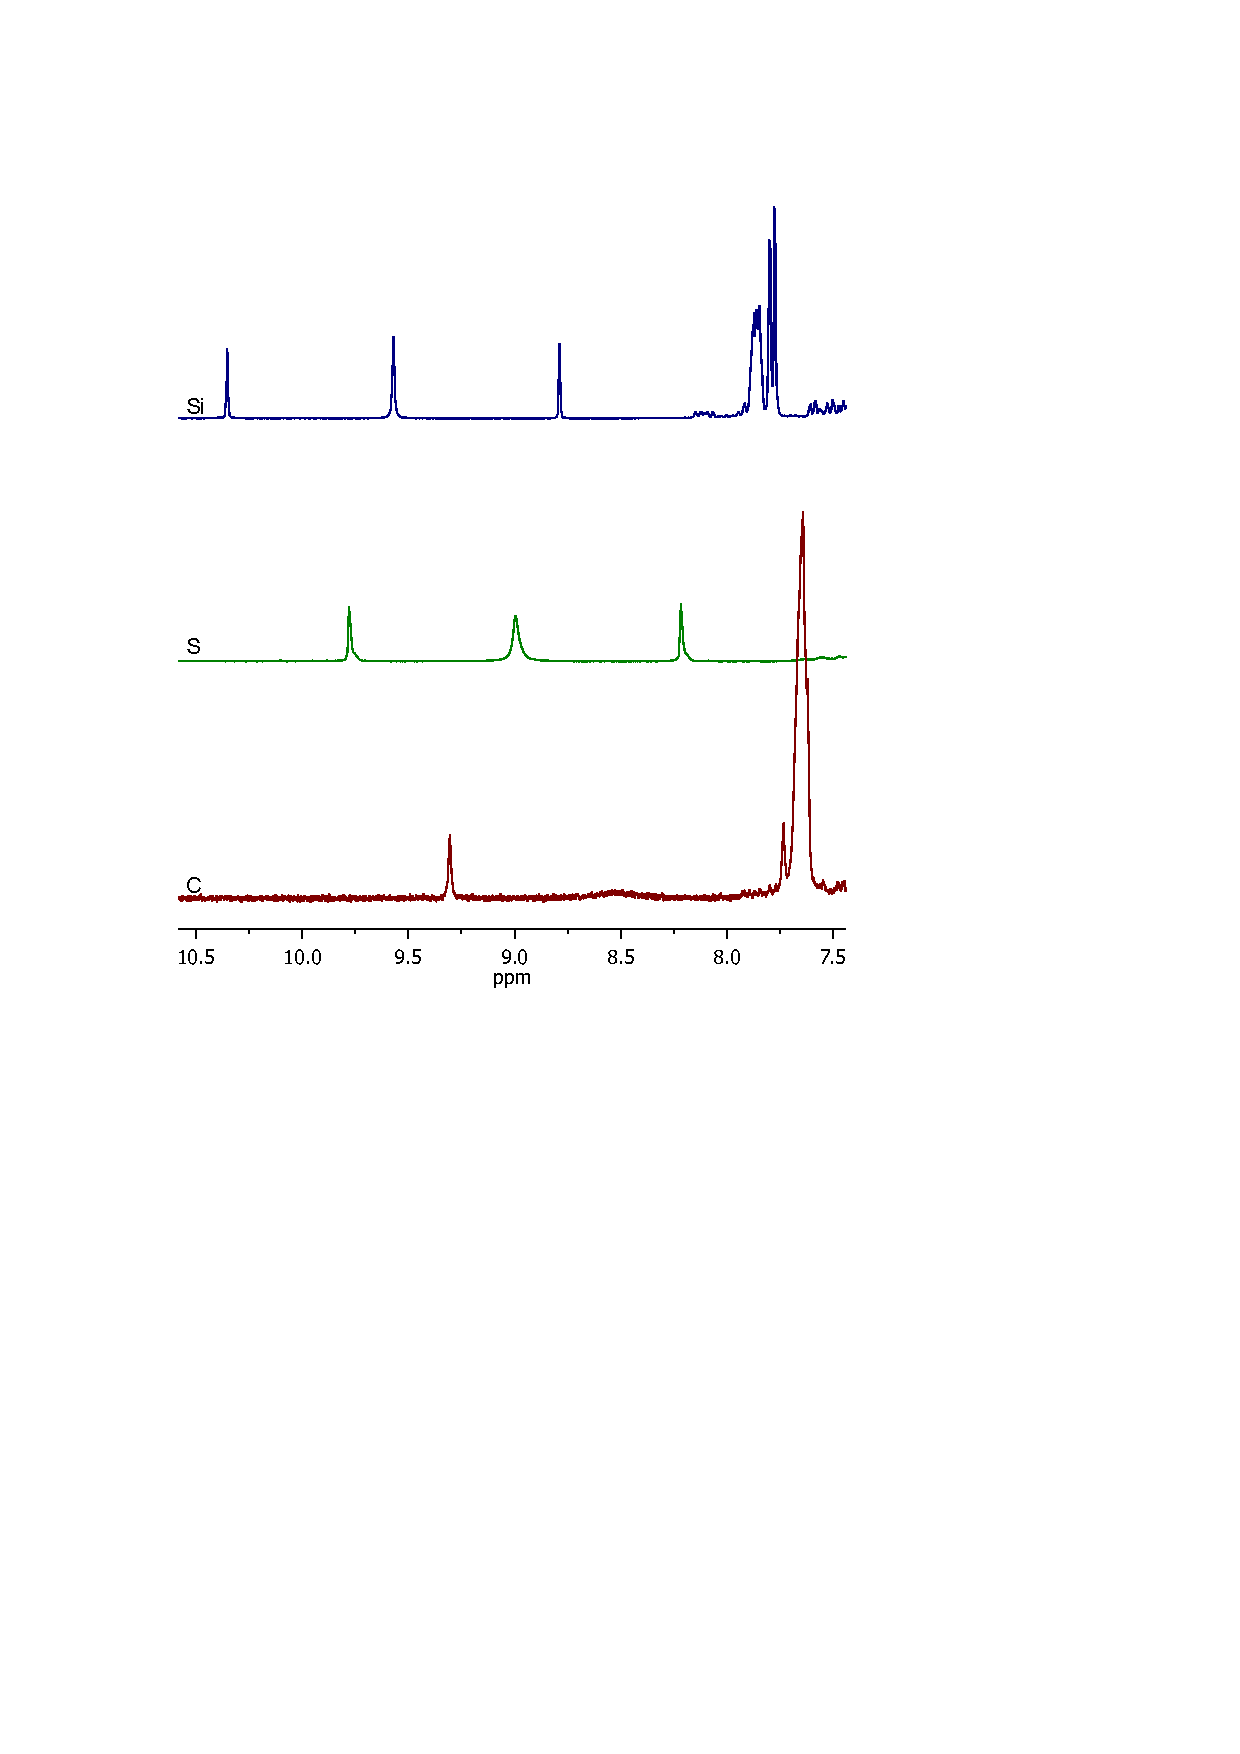
\includegraphics[scale=0.85]{../Figures/VTNMR/Protonatedligands.pdf}
%\caption[\proton{} NMR spectra for \tBusixantphos, \tButhixantphos{} and \tBuxantphos{} showing the P-H region]{\proton{} NMR spectra in \ce{CDCl3} at 20\degC{} for \tBusixantphos, \tButhixantphos{} and \tBuxantphos{} (Si, S and C respectively) showing the P-H region}
%\vspace{0.2cm}
%\label{Protonatedligandsnmr}
%\end{center}
%\end{figure}
%\vspace{0.2cm}

The dynamic behaviour of the phosphonium ions was further investigated using variable temperature \phosphorus{} and \proton{} NMR experiments on [(\tButhixantphos)H]\ce{CH\-(SO2CF3)2} (Figure \ref{VTStBuH}).  At room temperature a single peak is present in the \phosphorus{} NMR spectrum.  When heated this peak shifts slightly to higher ppm and becomes sharper.  This single peak indicates that the exchange of the proton between the two phosphorus atoms is occurring rapidly enough that the two phosphorus atoms appear to have the same environment on the NMR timescale.  Cooling below room temperature causes the singlet to broaden significantly, with coalescence occurring around -40\degC{}.  At -60\degC{} two broad signals are present.  One of these signals resolves into a doublet at -80\degC, however the other peak is still very broad ranging from 11--23 ppm.  Given that the protonation results in a downfield shift at room temperature, it is likely that the sharp doublet belongs to the unprotonated phosphorus and the broad peak is the protonated phosphorus.

%This is also consistent with the shift of the peaks at higher temperature where we observe a shift to higher ppm as the rate of exchange is increased.  \fixme{Kathryn says it's not likely)

\begin{figure}[h!]
\begin{center}
\vspace{0.5cm}
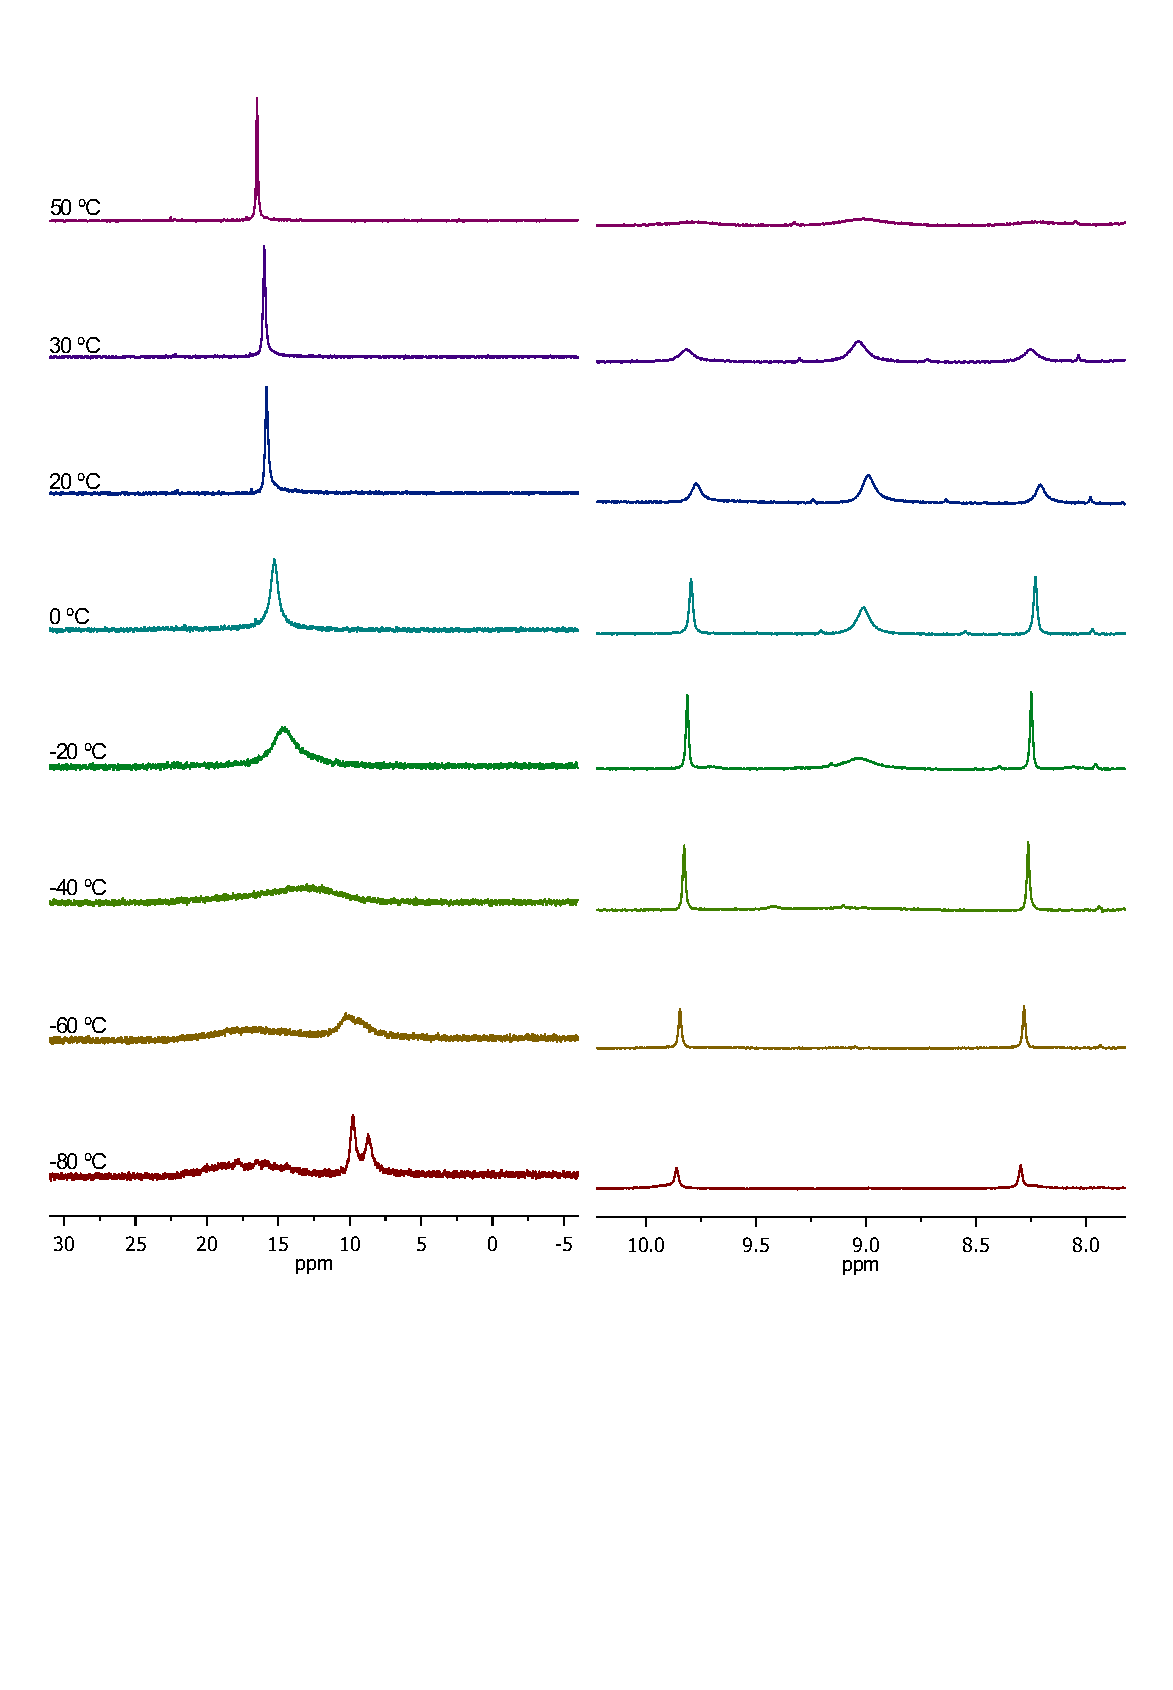
\includegraphics[scale=0.8, trim = 0cm 6.8cm 0cm 2cm]{../NMR/PhosphoniumVTNMRboth.eps}
\caption[VT-NMR for {[}(\tButhixantphos)H\ce{]+}]{Variable temperature \phosphorus{} (left) and \proton{} (right) NMR data for [(\tButhixantphos)H]\ce{CH(SO2CF3)2} in \ce{CD2Cl2}.}
\vspace{0.2cm}
\label{VTStBuH}
\end{center}
\end{figure}
\vspace{0.2cm}

%\begin{figure}[h!]
%\begin{center}
%\vspace{0.5cm}
%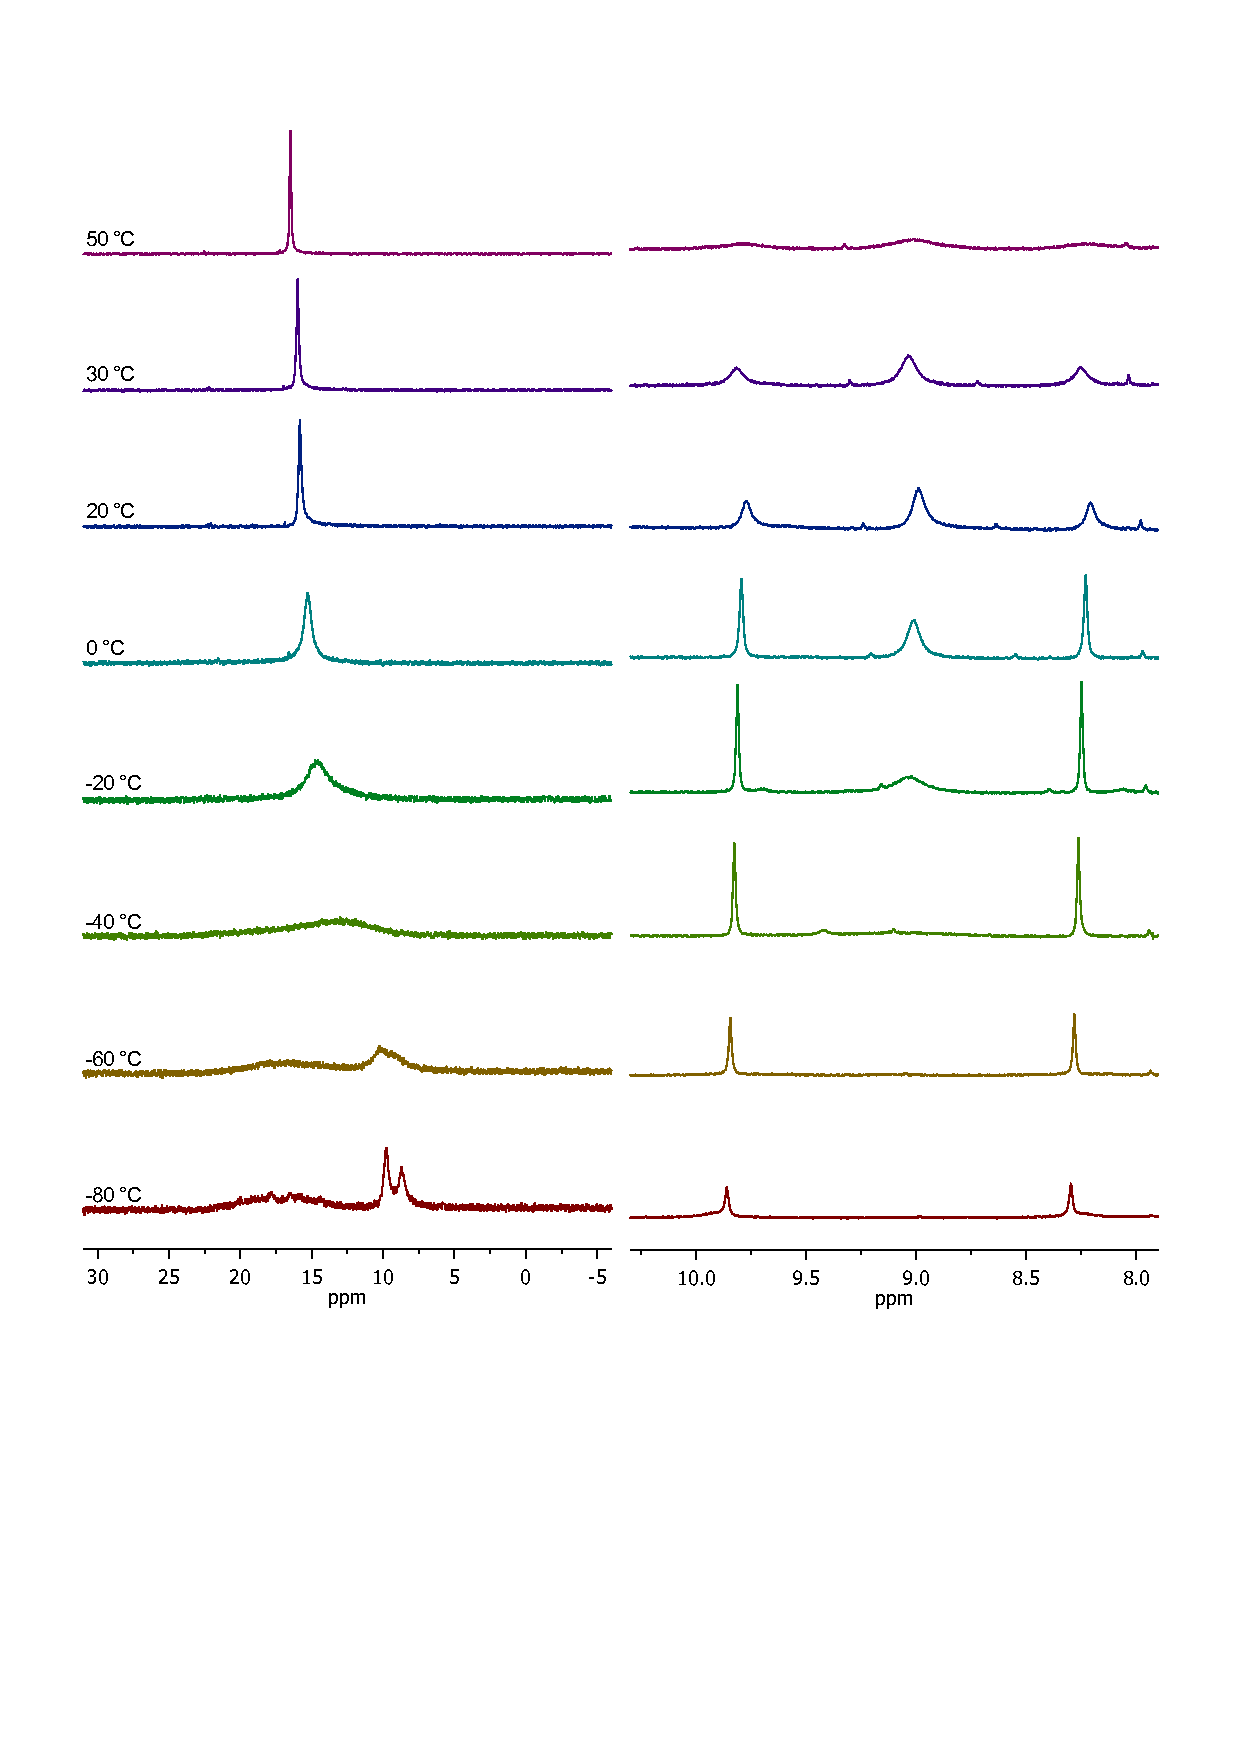
\includegraphics[scale=0.8]{../Figures/VTNMR/StBuHboth.pdf}
%\caption[Variable temperature \phosphorus{} and \proton{} NMR data for {[}(\tButhixantphos)H{]}\ce{CH(SO2CF3)2}]{Variable temperature \phosphorus{} (right) and \proton{} (left) NMR data for [(\tButhixantphos)H]\ce{CH(SO2CF3)2}}
%\vspace{0.2cm}
%\label{VTStBuH}
%\end{center}
%\end{figure}
%\vspace{0.2cm}

The variable temperature \proton{} NMR data for [(\tButhixantphos)\ce{H]CH(SO2CF3)2} (Figure \ref{VTStBuH}) shows similar changes to the \phosphorus{} NMR spectra.  At low temperature the proton is static on a single phosphorus atom so we observe a large doublet due to coupling with the phosphorus.  As the temperature increases to -20 \degC{}, a broad signal begins to appear in the centre of the doublet as exchange begins to occur and the signal changes from a simple doublet to a XAA\textprime{}X\textprime{} spin system.  The intensity of the central peak increases and at 20 \degC{} all three peaks begin to broaden again with coalescence at 50 \degC. This broadening may be the result of the proton no longer being isolated on a single molecule but delocalised across the entire system.   

Typically \phosphorus{} NMR spectra are proton decoupled.  However, with very strongly coupled systems such as phosphonium ions the decoupler is not able to fully decouple the spin system, resulting in broadening and side bands.  To further investigate the [(\tButhixantphos)\ce{H]CH(SO2CF3)2} system, proton-coupled phosphorus NMR spectra were obtained at room temperature and -80\degC{} (Figure \ref{VTStBuHcoupled}).  At room temperature a simple doublet appears, indicating rapid movement of the proton between the two phosphorus atoms thus coupling with both.  When cooled to -80\degC{}, the \phosphorus\{\proton\} spectrum showed a doublet and a broad singlet.  In the proton-coupled phosphorus spectrum, the doublet is retained confirming that this signal is for the non-protonated phosphorus which couples to the protonated phosphorus atom.  The broad singlet resolves into a doublet of doublets with coupling constants consistent with coupling to the proton and the other phosphorus.  This further confirms that no exchange of the proton is occurring at low temperature.  

\begin{figure}[htp]
\begin{center}
\vspace{0.5cm}
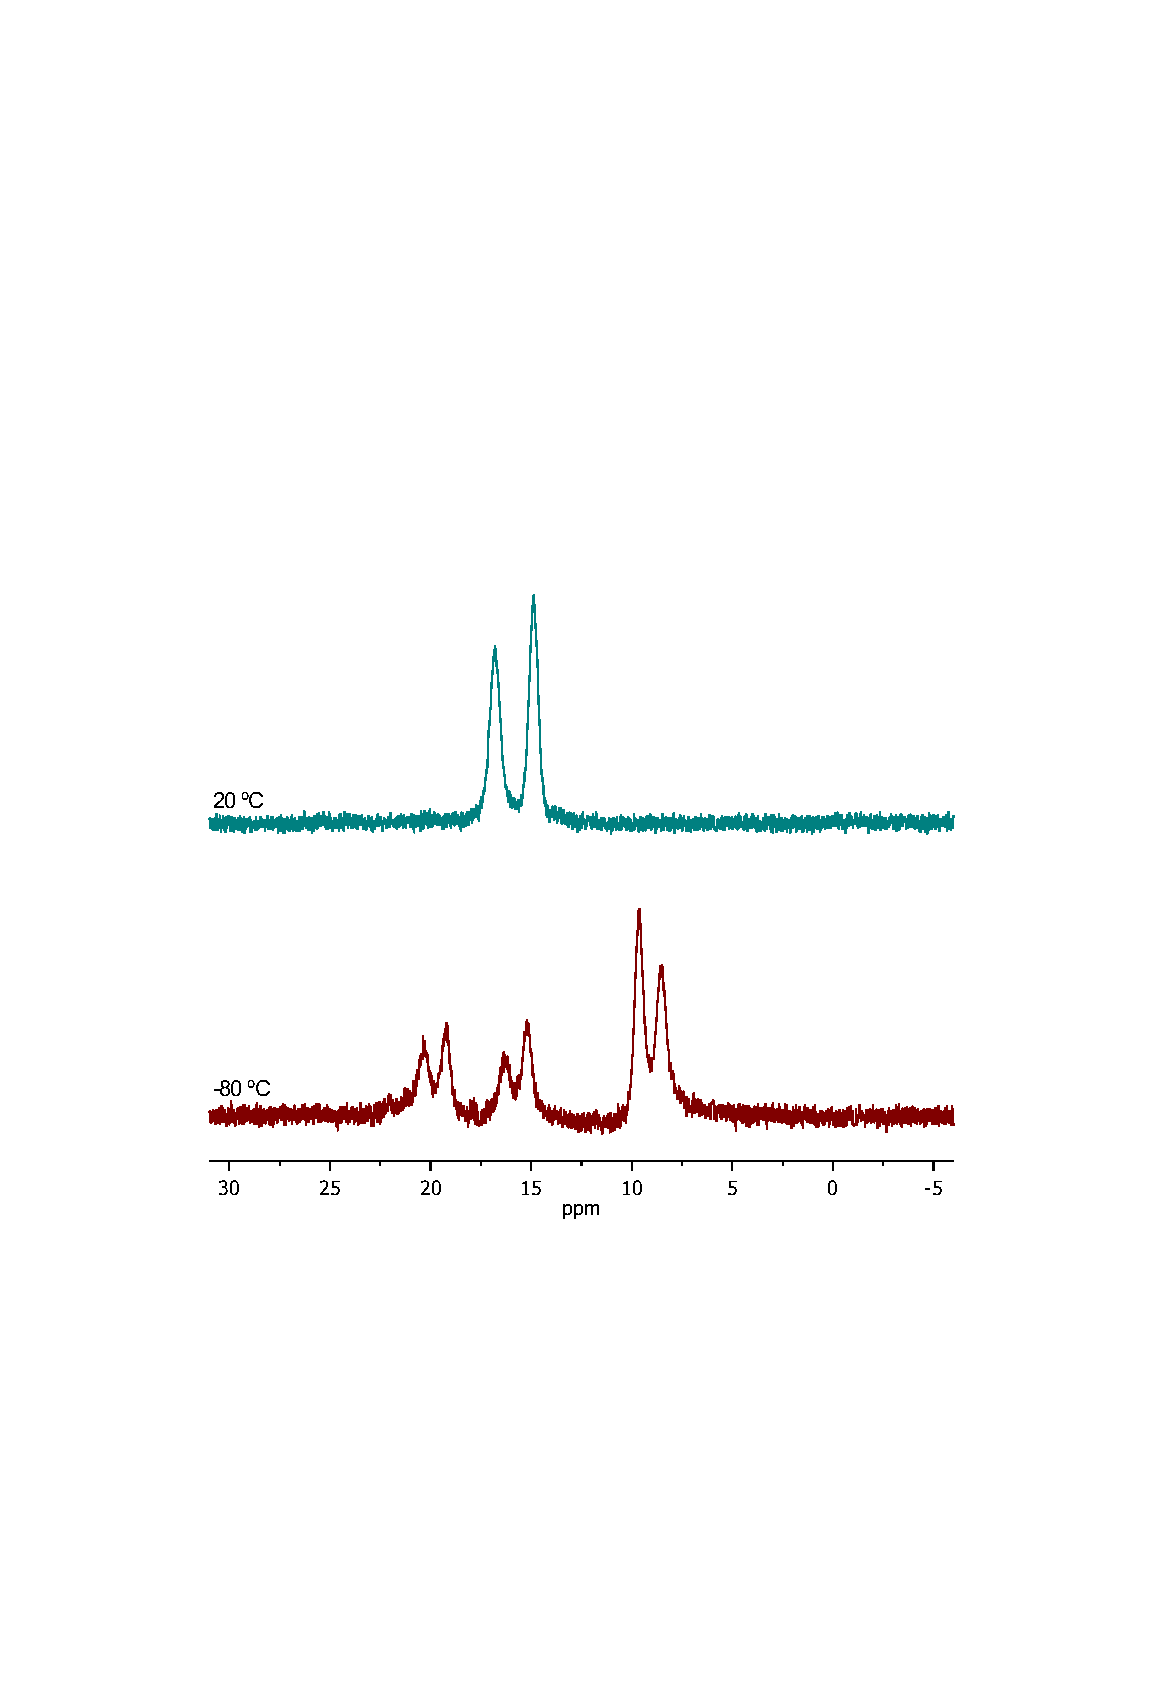
\includegraphics[scale = 0.8, trim = 0cm 8cm 0.5cm 10cm, clip]{../NMR/Coupledstacked.eps}
\caption[VT \proton-coupled \phosphorus{} NMR for [(\tButhixantphos\ce{)H]+}]{Variable-temperature proton coupled \phosphorus{} NMR data for [(\tButhixantphos\ce{)H]+} in \ce{CD2Cl2}.}
\vspace{0.2cm}
\label{VTStBuHcoupled}
\end{center}
\end{figure}  
\vspace{0.2cm}


%\begin{figure}[htp]
%\begin{center}
%\vspace{0.5cm}
%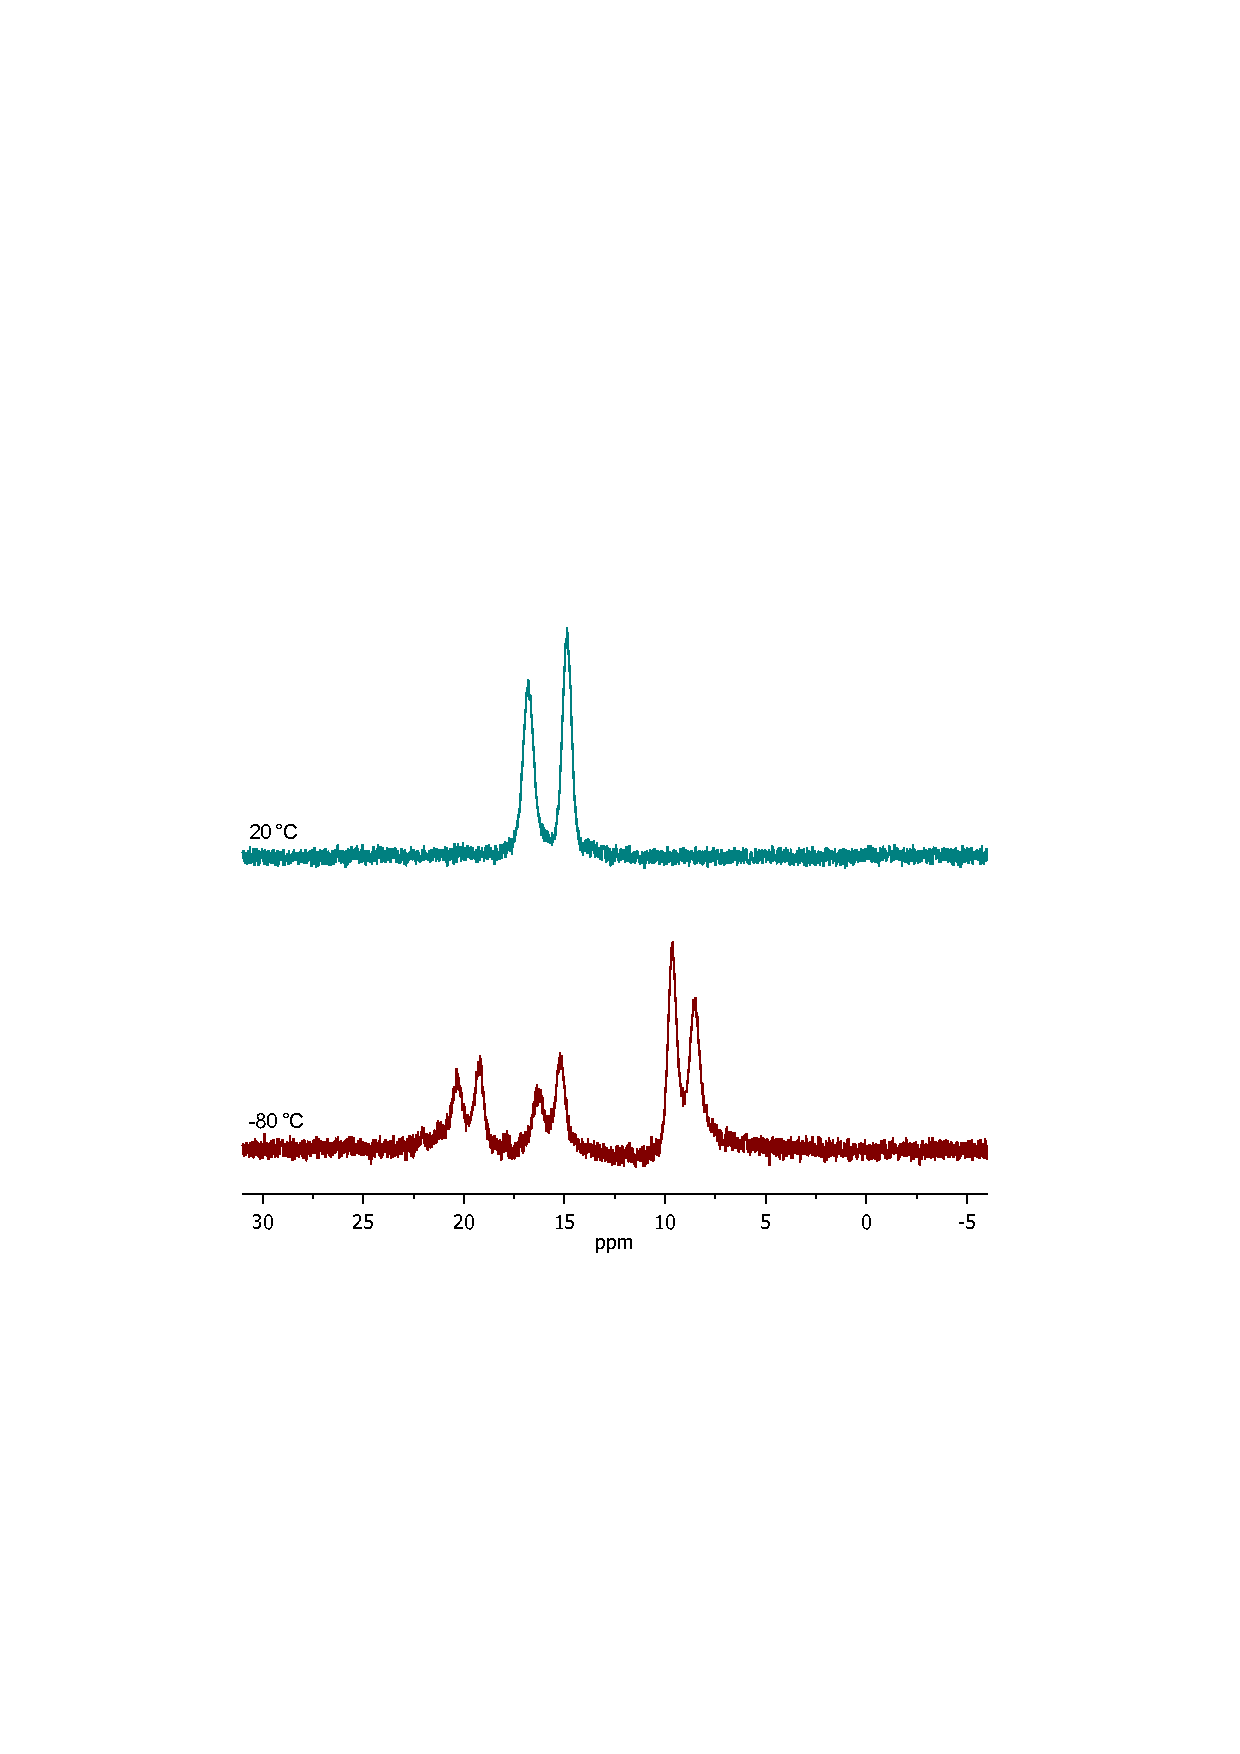
\includegraphics[scale=0.8]{../Figures/VTNMR/StBuHcoupled.pdf}
%\caption[Variable temperature proton coupled \phosphorus{} NMR spectra for (\tButhixantphos)H+]{Variable temperature proton coupled \phosphorus{} NMR data for (\tButhixantphos)H+}
%\vspace{0.2cm}
%\label{VTStBuHcoupled}
%\end{center}
%\end{figure}  
%\vspace{0.2cm}

%The protonation of the ligands was carried out using either or .  These are both strong acids with \pKa s of 2.0 and 2.4 in DMSO.\cite{Koppel2000}  The direct protonation of the ligands using a strong acid resulted in the phosphonium ions shown in Scheme \ref{Protonation}. 

%The degree of dynamism changes between the three ligands.  The sulfur bridged ligand with the smallest \biteangle{} has the greatest degree of exchange between the systems \fixme{can I get temperatures for coalescence as this would prove it nicely}.  \fixme{the S has the middle one need to check how much coupling in the carbon one}  The sulfur bridged ligand has very little coupling evident in the NMR spectra compared to the silicon bridged ligand which has a number of clearly defined coupled peaks.  The silicon bridged ligand has the largest degree of exchange at room temperature as the phosphorus atoms are held much closer - as shown by the smaller \biteangle{} which would indicate a greater degree of interaction between the tertiary phosphine and the phosphonium ion and thus much more rapid exchange.  As such at room temperature we are below coalescence and thus the NMR peaks resolve into much clearer signals than those found with the sulfur or carbon bridged systems.

%Likewise the carbon bridged system with the largest \biteangle{} will have the smallest degree of exchange at room temperature.  Hence we are closer to coalescence than in the other two so the NMR spectra are very broad and unable to be fully assigned.  \fixme{check the NMR data for 3013 on 600 MHz}

%Variable temperature phosphorus and proton NMR data for is shown in Figures \ref{VTStBuHphosphorus} and \ref{VTStBuHproton}

Single colourless crystals of [\tButhixantphos(H)]\ce{CPh(SO2CF3)2} suitable for X-ray diffraction were grown from the reaction mixture in benzene.  The compound crystallised with a benzene solvate, as 2[\tButhixantphos{}\ce{(H)]CPh(SO2CF3)2}$\cdot{}$\ce{C6D6} in the monoclinic space group \emph{P}2\sub{1}/\emph{n}.  Selected bond lengths and angles are summarised in Table \ref{table:crystalprotonated:lengths}, and crystallographic data is given in Table \ref{table:crystalprotonated:data}.  Although the cationic portion was well refined, one of the counterions is disordered with two positions for the \ce{SO2CF3} chains.  The proton on the phosphonium ion was able to be found and is exclusively located on a single phosphorus atom.  As a result the \gls{esd} on the bond lengths and angles involving this proton are relatively high.  The distances from the proton to the other phosphorus or to the oxygen atom are both too long to indicate any degree of interaction.  The crystal structure was collected at 284.87 K, and based on the variable temperature NMR data significant exchange of the proton is expected at this temperature.  However, this is not apparent in the X-ray structure suggesting that the exchange does not occur in the solid state.  

\begin{figure}[hp!]
\begin{center}
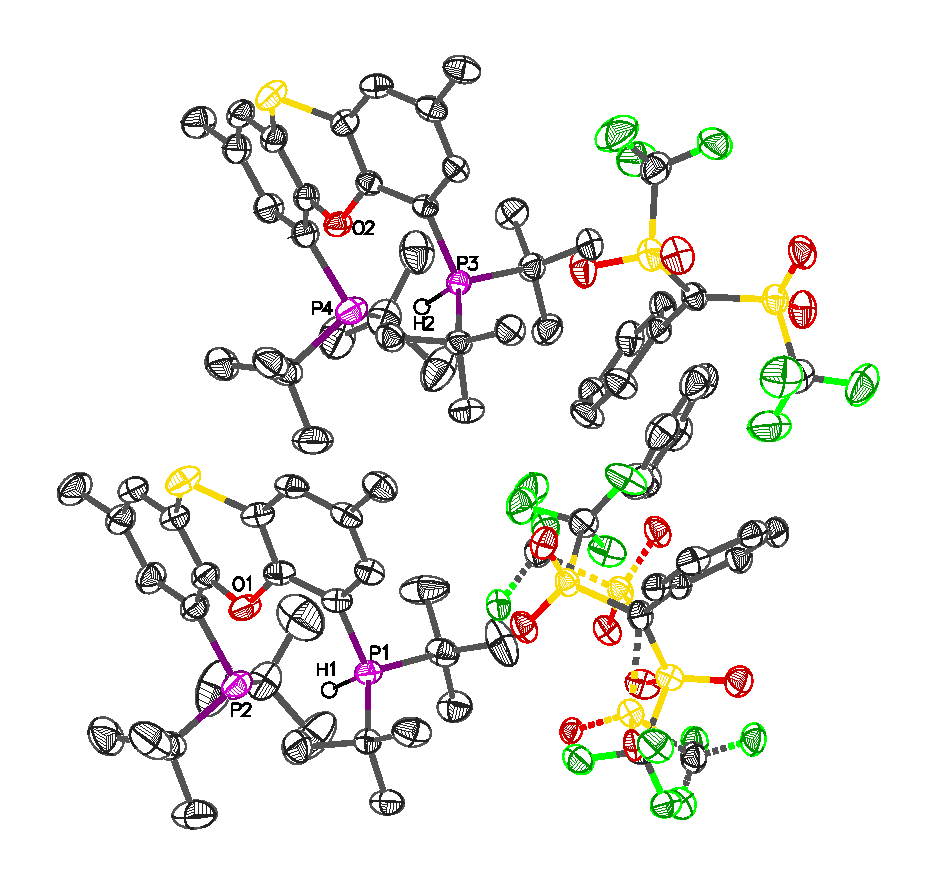
\includegraphics{../Crystalstructures/mrmnb.eps}
\caption[X-ray crystal structure of {[}(\tButhixantphos)H{]}\ce{CPh(SO2CF3)2}]{X-ray crystal structure of 2{[}(\tButhixantphos)H{]}\ce{CPh(SO2CF3)2}$\cdot{}$ \ce{C6D6} (50\% probability thermal ellipsoids).  Selected hydrogen atoms omitted for clarity.}
\label{Crystalprotonated}
\end{center}
\end{figure}

\begin{table}[htp]
\small
\caption[Selected bond distances (\AA) and angles (\degrees) of 2[(\tButhixantphos)\ce{H]CPh(SO2CF3)2}$\cdot{}$ \ce{C6D6}]{Selected bond distances (\AA) and angles (\degrees) of 2[(\tButhixantphos)\-\ce{H]CPh(SO2CF3)2}$\cdot{}$ \ce{C6D6}.}
\vspace{1em}
\label{table:crystalprotonated:lengths}
\begin{center}
\begin{tabular}{l l l l l}
	\toprule
	\multicolumn{2}{l}{\bfseries{~Bond distances (\si{\angstrom})}} &~~~& \multicolumn{2}{l}{\bfseries{Bond angles (\degrees)}} \\
	\midrule		
	P1-H1	& 1.22(3)		&~~~& P1-H1...P2	& 160(2)\\
	P2...H1	& 2.96(3)		&~~~& P1...O1...P2	& 89.19(6)\\
	P1...P2	& 4.1290(11)	&~~~& P3-H2...P4	& 154(2)\\
	O1...H1	& 2.44(3)		&~~~& P3...O2...P4	& 86.40(5)\\
	P3-H2	& 1.22(3)		&~~~& Ring 1...Ring 2 & 18.28(10)\\
	P4...H2	& 2.91(3)		&~~~& Ring 3...Ring 4 & 26.67(10)\\
	P3...P4	& 4.0372(11)	&~~~& ~			& ~\\
	O2...H2	& 2.43(3)		&~~~& ~			& ~\\
	\bottomrule{}
\end{tabular}
\end{center}
\end{table}

\begin{table}[htp]
\small
\caption[Crystallographic data of 2[\tButhixantphos(H){]}\ce{CPh(SO2CF3)2}$\cdot{}$\ce{C6D6}]{Crystallographic data and structure refinement of 2[\tButhixantphos(H)]\ce{CPh(SO2CF3)2}$\cdot{}$\ce{C6D6}} 
\vspace{1em}
\label{table:crystalprotonated:data}
\small
\begin{center}
\begin{tabular}{l l}
	\toprule
	\bfseries{Empirical formula}~~& \bfseries{\ce{C84H110F12O10P4S6}}\\
	\midrule
	Formula weight	 							& 1823.95\\
	Temperature/K	 							& 284.87(10)\\
	Crystal system	 							& monoclinic\\
	Space group	 							& P21/n\\
	a$/$\si{\angstrom}							& 14.19615(12)\\
	b$/$\si{\angstrom} 							& 39.4563(3)\\
	c$/$\si{\angstrom}							& 16.35832(15)\\
	$\alpha/$\degrees							& 90\\
	$\beta/$\degrees							& 100.1751(8)\\
	$\gamma/$\degrees							& 90\\
	Volume$/$\si{\angstrom\cubed}  				& 9018.64(13)\\
	Z	 									& 4\\
$\rho$\sub{calc} \si{\milli\gram}$/$\si{\milli\metre\cubed} 	& 1.343\\
\si{\metre}$/$\si{\milli\metre} 							& 2.749\\
F(000)	 									& 3832.0\\
Crystal size$/$\si{\milli\metre\cubed}	 				& 0.49 x 0.16 x 0.14\\
Radiation	 									& CuK$\alpha$ ($\lambda$ = 1.54184)\\
2$\theta$ range for data collection					& 5.928 to 147.832\degrees\\
Index ranges	 								& -17 $\leq$ h $\leq$ 17, -48 $\leq$ k $\leq$ 48, -20 $\leq$ l $\leq$ 20\\
Reflections collected	 							& 69203\\
Independent reflections	 						& 17960 [R\sub{int} = 0.0261, R\sub{sigma} = 0.0219]\\
Data$/$restraints$/$parameters					& 17960$/$291$/$1221\\
Goodness-of-fit on F$^{2}$	 					& 1.068\\
Final R indexes [I$>$=2$\sigma$ (I)]	 				& R\sub{1} = 0.0549, wR\sub{2} = 0.1473\\
Final R indexes [all data]	 						& R\sub{1} = 0.0623, wR\sub{2} = 0.1531\\
Largest diff. peak/hole / e \si{\per\angstrom\cubed}		& 1.11/-0.56	\\
	\bottomrule
\end{tabular}
\end{center}
\end{table}

\section{Selenides}
\label{section:selenides}

The electronic properties of phosphine ligands can be investigated in a number of different ways.  The most well-known quantification is the Tolman electronic parameter.\cite{Tolman1970}  This involves the measurement of the carbonyl stretching frequency in a \ce{[Ni(CO)3L]} complex.  Related approaches use [Mo\ce{(CO)5L}] or [Rh(CO)Cl\ce{L2}] complexes.\cite{Roodt2003, Banger2009}  The value of the phosphorus-metal coupling constants in platinum or rhodium complexes have also been used to quantify the electronic properties of phosphine ligands.\cite{Mann1980, Pregosin2012, Roodt2003, Banger2009}  The values of the carbonyl stretching frequency and the phosphorus-metal coupling constants are dependent on the geometries of the metal complexes and these can be influenced significantly by steric properties, such as those imposed by large diphosphine ligands.  The \JPSe{} spin-spin coupling constants of phosphine selenides are a convenient and accurate measure of the electronic properties of tertiary phosphines.\cite{Beckmann2011, Muller2008c, Anderson2001} In this case the more electron donating the phosphorus substituents are, the lower the resulting \JPSe{}.  

The phosphine selenides are air-stable solids that are generally relatively straightforward to synthesise by reaction of the phosphine with either elemental selenium or potassium selenocyanide (with or without heating).\cite{Beckmann2011, Bungu2007}  The value of \JPSe{}, as with all coupling constants, is governed by interactions between the s-orbitals.  According to Bent's rule ``atomic s-character concentrates in orbitals directed towards electropositive substituents''.\cite{Bent1961}  Thus the greater the value of \JPSe{} the more s-character is present in the P-Se bond, indicating a greater degree of electronegative substituents, and thus the less electron donating the phosphine ligand will be.

% It is not possible to completely eliminate steric influences on the \JPSe{}, as selenium has a significant steric and electronic impact resulting in repulsion of the two phosphino-selenides.  This has been noted as the mono- and di-selenides of diphosphines often have different coupling constants.  In these cases the mono-selenide generally gives a better description of the electronic influence of the diphosphine.  

%Numerous approaches to studying the steric influence of tertiary mono and diphosphine ligands exist, the most prolific are the Tolman cone angle\cite{Tolman1977} and the natural bite-angle\cite{Casey1990}.  The electronic influence are less well defined, typical approaches involve the CO stretching frequency of metal carbonyl complexes, or analysis of \oneJPM{} spin-spin coupling constants.  However, the coupling constants are highly dependent on the geometries of metal complexes and this can be influenced significantly by steric properties, such as those imposed by large diphosphine ligands.  

%The \JPSe{} coupling constant has shown to correlate relatively well with the Tolman electronic parameter.\cite{Allman1982}  Furthermore the phosphino-selenides are 
%
%Using the phosphino-selenides to investigate the electronic properties of the phosphine also avoids the expensive transition metals used in other methods.  The resulting phosphino-selenides are air-stable as compared to metal carbonyl complexes which often decompose if not stored under carbon monoxide.   Using elemental selenium in the synthesis also avoids the use of toxic gases (although this is not the case for potassium selenocyanide which produces potassium cyanide as a by-product which will react rapidly with any proton source to form hydrogen cyanide).  

In addition to the use of \JPSe{} as a measure of the electronic influence of a phosphine, it can also be used to measure the Br\o{}nsted basicity of a given phosphine.  A correlation between the experimentally measured \pKb{} and the \JPSe{} value has been reported with linear regression: \JPSe{} = 7.60 $\times{}$ \pKb{}~+~646~(R\superscript{2} = 0.9492).\cite{Beckmann2011}  As such, determining the value of \JPSe{} allows for calculation of the \pKb{} and has shown good agreement with the experimentally determined data.  One limitation of this method is the impact that sterically bulky groups can have.  For \ce{P^{t}Bu3} the correlation suggests a \pKb{} value of 6.0 however the experimentally determined value is 2.60.\cite{Beckmann2011}  This is the result of the \tBu{} groups increasing the C-P-C angles, thus decreasing the s-character of the lone pair of electrons.

The \tBuxantphos{} ligands showed significant resistance to selenation.  Reaction directly with elemental selenium has been reported as preferable to potassium selenocyanide as the latter reacts slowly and gives lower yields.\cite{Beckmann2011}  The previously reported \Phxantphos{} diselenide was synthesised by refluxing \Phxantphos{} and red selenium in toluene overnight resulting in diselenation.\cite{Jahromi2012}  Attempting this method with the \tBuxantphos{} ligands reported here showed little reaction.  Attempts were also made using KSeCN similar to those previously reported, \cite{Bungu2007} however these were also unsuccessful.  Successful monoselenation was obtained by refluxing the ligands with a large excess of grey selenium in toluene for three days (Scheme \ref{Selenation}).  Extending the reaction period did not result in the formation of any diselenide.  This is likely due to the steric restraints of these ligands.

\begin{scheme}[htbp]
\begin{center}
\vspace{0.5cm}
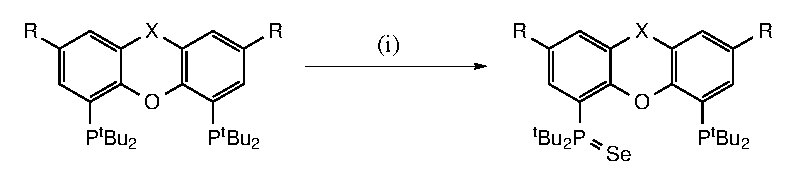
\includegraphics{../Schemes/Selenation.eps}
\caption[Selenation of \tBuxantphos{} ligands]{Selenation of \tBuxantphos{} ligands, (X = \ce{CMe2}, R = H), \tButhixantphos{} (X = S, R = Me) and \tBusixantphos{} (X = \ce{SiMe2}, R = H).  \emph{Reagents and conditions:} (i) Se, reflux, toluene, 3 days.}
\vspace{0.2cm}
\label{Selenation}
\end{center}
\end{scheme}
\vspace{0.2cm}

%The \phosphorus{} NMR spectra of the three phosphino-selenides showed significant differences.  For \tBuxantphos{} selenide two clear peaks were observed in a 1:1 ratio clearly indicating the formation of the monoselenide.  For \tButhixantphos{} and \tBusixantphos{} multiple peaks were observed though only one in the region expected for an non-selenated phosphine.  There were two moderately broad peaks at higher ppm close to where the selenated phosphorus of \tBuxantphos{} selenide appeared.  Variable temperature \phosphorus{} NMR showed that the ratio of these peaks changed at low temperature \fixme{add the spectra} leading us to propose the presence of two distinct rotamers.  

%These rotomers were investigated using density functional theory (DFT) using the B3LYP functional and TZVP basis set.  Two rotamers (representative structures shown for \tButhixantphos{} shown in Figure \ref{Seleniderotomers} were found as minima for all three ligands, with very close energy values thus indicating little difference between the two.  However, it is likely the a significant barrier to interconversion exists due to the steric restraints of the system.  

% The \JPSe{} values vary across a range of 12 Hz.  The \JPSe{} values for \tBuxantphos{} and \tButhixantphos{} are similar, with a difference of 1.4 Hz; whilst \tBusixantphos{} has a much smaller \JPSe{} value (Table \ref{table:selenides}).  

The cleanest reaction was observed between \tBuxantphos{} and selenium, with a single asymmetric product observed.  For \tButhixantphos{} and \tBusixantphos{} a single major product was observed, again consistent with monoselenation. Selected NMR data for the selenides is given in Table \ref{table:selenides}.  The \phosphorus{} NMR spectra each show two peaks in a 1:1 ratio.  One peak is shifted only slightly (0.4--7.5 ppm) from the starting material while the other peak is shifted significantly (91.7--94.3 ppm upfield).  The asymmetry and the change in chemical shift of only one of the \phosphorus{} NMR signals indicates the formation of the monoselenide.  The \JPSe{} values are similar for the three ligands with a range of 12 Hz.  The monoselenated \tButhixantphos{} derivative was found to have \JPSe{} = 698.5 Hz, while the monoselenated \tBuxantphos{} has \JPSe{} = 696.3 Hz.  These are much lower than that reported for xantphos selenide (749 Hz)\cite{Jahromi2012}.  This lower coupling constant is expected as \emph{tert}-butyl groups are more electron donating than phenyl substituents.

\begin{sidewaystable}[htbp]
\caption[Selected \phosphorus{} NMR data for \tBuxantphos{} selenides]{Selected \phosphorus{} NMR data for \tBuxantphos{} selenides in 1:1 CDCl3:CD2Cl2}
\vspace{1em}
\label{table:selenides}
\small
\begin{center}
\begin{tabular}{l c c c c c c}
	\toprule
	\bfseries{Diphosphine} & \bfseries{\phosphorus{} (P $/$ppm)} & \bfseries{P $\Delta\delta/$Hz} &\bfseries{\phosphorus{} (P=Se $/$ppm)} & \bfseries{P=Se $\Delta\delta/$Hz} & \bfseries{\JPSe (Hz)} & \bfseries{\pKb} \\
	\midrule		
	\tBuSixantphos		&15.9	& 7.5 	& 102.7	& 94.3	& 689.1	& 5.67\\
	\tBuThixantphos	&11.7	& 2.2		& 103.7	& 94.2	& 698.5	& 6.90\\
	\tBuXantphos		&10.6	& 0.4		& 101.9	& 91.7	& 697.1	& 6.72\\
	\bottomrule{}
\end{tabular}
\end{center}
\end{sidewaystable}

Using the correlation reported by Beckmann \emph{et al.,} it is possible to convert the values of \JPSe{} for the \tBuxantphos{} selenides and the previously reported \Phxantphos{} diselenide into \pKb{} values.\cite{Jahromi2012}  The \pKb{} values for the \tBuxantphos{} ligands range between 5.67 and 6.90 which fall between the \ce{PPhMe2} and \ce{PMe3}.\cite{Beckmann2011}  This is consistent with expectations as \tBu{} groups are more electron donating than methyl groups while the phenyl still results in a higher \pKb{} than those for the trialkyl phosphines.  The \pKb{} value for \Phxantphos{} is 13.55, indicating that the \tBuxantphos{} ligands are significantly more basic.  This significant difference is expected as tert-butyl groups are strongly electron donating whilst phenyl substituents are electron withdrawing.\cite{Tolman1977}  This effect will dominate any other subtle effects that may arise due to bite-angle or steric considerations.  
  
The bite-angle may play a role in the value for the \JPSe{} coupling constant as monoselenide diphosphines have shown through space coupling to the other phosphorus.\cite{Hierso2014}  This would result in a lower \JPSe{} value than otherwise expected and the effect would be more pronounced with smaller bite-angles.  In this case \tBusixantphos{} has the lowest \pKb{} of the three ligands and also the smallest bite-angle, so a bite-angle effect may be present.  However, the differences cannot be purely the result of the bite-angle as \tButhixantphos{} has the largest \JPSe{} value but \tBuxantphos{} has the largest bite-angle.

In addition to the influence of the bite-angle on the \JPSe{} coupling constant there must exist another electronic effect contributing to the difference between the ligands.  Both \tButhixantphos{} and \tBuxantphos{} groups have an \emph{ortho} ether and a \emph{meta} alkyl group, in addition \tButhixantphos{} has the thioether bridge.  Thioethers are electron donating by resonance, but being in the \emph{meta} position to the phosphorus the negative charge that could be generated is unable to interact with the phosphorus atom.  With sulfur being slightly more electronegative than carbon, a thioether is also slightly inductively electron withdrawing, which would result in the phosphorus being very slightly less basic in the case of \tButhixantphos{} when compared to \tBuxantphos{}.

\section{Concluding Remarks}

Two new \tBuxantphos{} ligands, \tBusixantphos{} and \tBuxantphos{} have been synthesised and an alternate synthesis of \tBuxantphos{} has been reported by lithiation of the appropriate backbone using \emph{sec}-butyllithium with \gls{TMEDA} and treatment with \ce{P^{t}Bu2Cl}.  Although this method requires long reactions times the only by-product is the mono-phosphine which can undergo the same process again to generate higher yields.  NMR analysis of the three ligands showed a XAA\textprime{}X\textprime{} spin system for the \tBu{} protons, suggestive of through-space coupling of the two phosphorus atoms.

Natural bite-angles of 126.80, 126.98, and 127.56\degrees{} were calculated using DFT for the \tBusixantphos{}, \tButhixantphos, and \tBuxantphos{} respectively.  For comparative purposes the bite-angles for the \Phxantphos{} ligands were also calculated: \Phsixantphos{} (111.89\degrees), \Phthixantphos{} (\fixme{112.65\degrees}), and \Phxantphos{} (114.18\degrees).  The values for the \Phxantphos{} ligands are slightly larger than those calculated using molecular mechanics, though the value for \tBuxantphos{} is lower than the previously reported value (140\degrees) calculated with molecular mechanics.  This is likely due to the molecular mechanics value overestimating the steric impact of the \tBu{} substituents.  A comparison of the natural and median crystallographic bite-angles for a range of different diphosphine ligands showed a good correlation between the two, indicating that the natural bite-angles can be excellent predictors of coordination behaviour.  

The three \tBuxantphos{} ligands react rapidly with one equivalent of acid to generate [(\tBuxantphos)H]\ce{CH(SO3CF3)2}.  The proton moves between the two phosphorus atoms at in room temperature solutions.  This process was investigated using proton-coupled \phosphorus{} NMR spectroscopy and low temperature \proton{} and \phosphorus{} NMR spectroscopy, revealing that the proton is isolated on a single phosphorus below -40\degC.  The X-ray crystal structure of [(\tButhixantphos)H]\ce{CPh(SO3CF3)2} was obtained, and the phosphonium proton was able to be located: isolated on a single phosphorus.  

The electronic properties of the \tBuxantphos{} ligands were investigated by the synthesis of phosphine selenides.  In all cases the monoselenide formed with no evidence for a diselenide.  The values of \JPSe{} ranged from 689.1--698.5 Hz, which was converted into \pKb{} values of 5.67--6.90.  These fall between the values of \ce{PPh2Me} and \ce{PMe3} which is consistent with the strong electron donation from the \tBu{} substituents and the electron withdrawing nature of the aryl backbone.  The \pKb{} value for \Phxantphos{} is 13.55 showing the difference in the electrons behaviour of the \tBuxantphos{} ligands.

Overall this chapter provides an interesting introduction into the chemistry of the \tBuxantphos{} ligands and suggests that the coordination chemistry may be different to that of the \Phxantphos{} ligands as a result of the much larger natural bite-angles and more electron-rich phosphorus atoms.  














